%!TEX root = ../thesis.tex
\chapter{盾构隧道服役性能预测}
\label{chap:prediction}

第~\ref{chap:tsi}~章主要介绍了如何采用当前的观测变量,对盾构隧道服役性能进行评估,由第~\ref{chap:tsi}~章的基本假设可知,TSI计算仅考虑当前时间点的数据,有时候根据已有数据对未来数据的预测同样很重要。对于盾构隧道监测和病害数据,有两个重要的维度:时间和空间。时间维度是指单一点的数据随着时间的发展而变化,空间维度是指不同监测点数据并不是独立的,例如临近的沉降点监测数据应该是相似,不同监测点数据之间存在空间关联性。本章主要内容是在历史监测数据基础上,建立时空数据的预测模型,为隧道服役性能预测提供支持。

本章采用时间序列(Time Series)方法对隧道数据进行预测,时间序列可以用于研究事物随时间的发展规律,是一种定量分析方法。时间序列认为数据与时间之间存在关联性,数据之间也具有前后相承的联系,同时数据因为各种外部原因还表现出随机性。时间序列的主要思想是采用历史数据和外部影响因素近似描述不同类型的时序数据,并建立稳定的模型从而预测数据的未来发展趋势。一组有序的数列:${{Y}_{1}},{{Y}_{2}},{{Y}_{3}}\cdots {{Y}_{t}}$(其中$t$代表时间序号),时间间隔均匀的,且是随机过程的一个实现,则该序列为时间序列。在本章开始之前,先介绍序列的一些基本概念。

(1)指标集$T$

指的是时间$t$的取值范围,对于随机过程,$t$是连续变化的,对于时间序列,$t$则是离散的,取$t$为$\left\{ 0,\pm 1,\pm 2,\pm 3\cdots  \right\}$,在实际中,$t$一般取$\left\{ 0,1,2,3\cdots  \right\}$。

(2)采样间隔$\Delta t$

即时间序列相邻数据之间的时间差,一般地时间序列分析要求数据采样间隔是一致的。

(3)平稳时间序列

大部分时间序列分析要求数据为平稳时间序列。定义为如果对于$\forall {{t}_{1}},{{t}_{2}},{{t}_{3}}\cdots {{t}_{n}}$,$h\in T$和任意的$n$,都有$\left( {{Y}_{{{t}_{1}}}},{{Y}_{{{t}_{2}}}}\cdots {{Y}_{{{t}_{n}}}} \right)$与$\left( {{Y}_{{{t}_{1}}+h}},{{Y}_{{{t}_{2}}+h}}\cdots {{Y}_{{{t}_{n}}+h}} \right)$同分布,则称该时间序列为平稳时间序列。

(4)白噪声序列

白噪声序列是特殊的平稳序列。定义为互相独立的序列变量$\left\{ {{Y}_{t}} \right\}$,对于任意$s\ne t$,如果$Cov({{Y}_{s}},{{Y}_{t}})=0$,则称该序列为白噪声序列。也即是说,白噪声序列在不同的时间点上的数据的协方差为0,无法采用历史数据来预测未来的数据,未来数据是无规律的。

\begin{figure}[htb!] 
    \centering 
    \begin{tabular}{c} 
        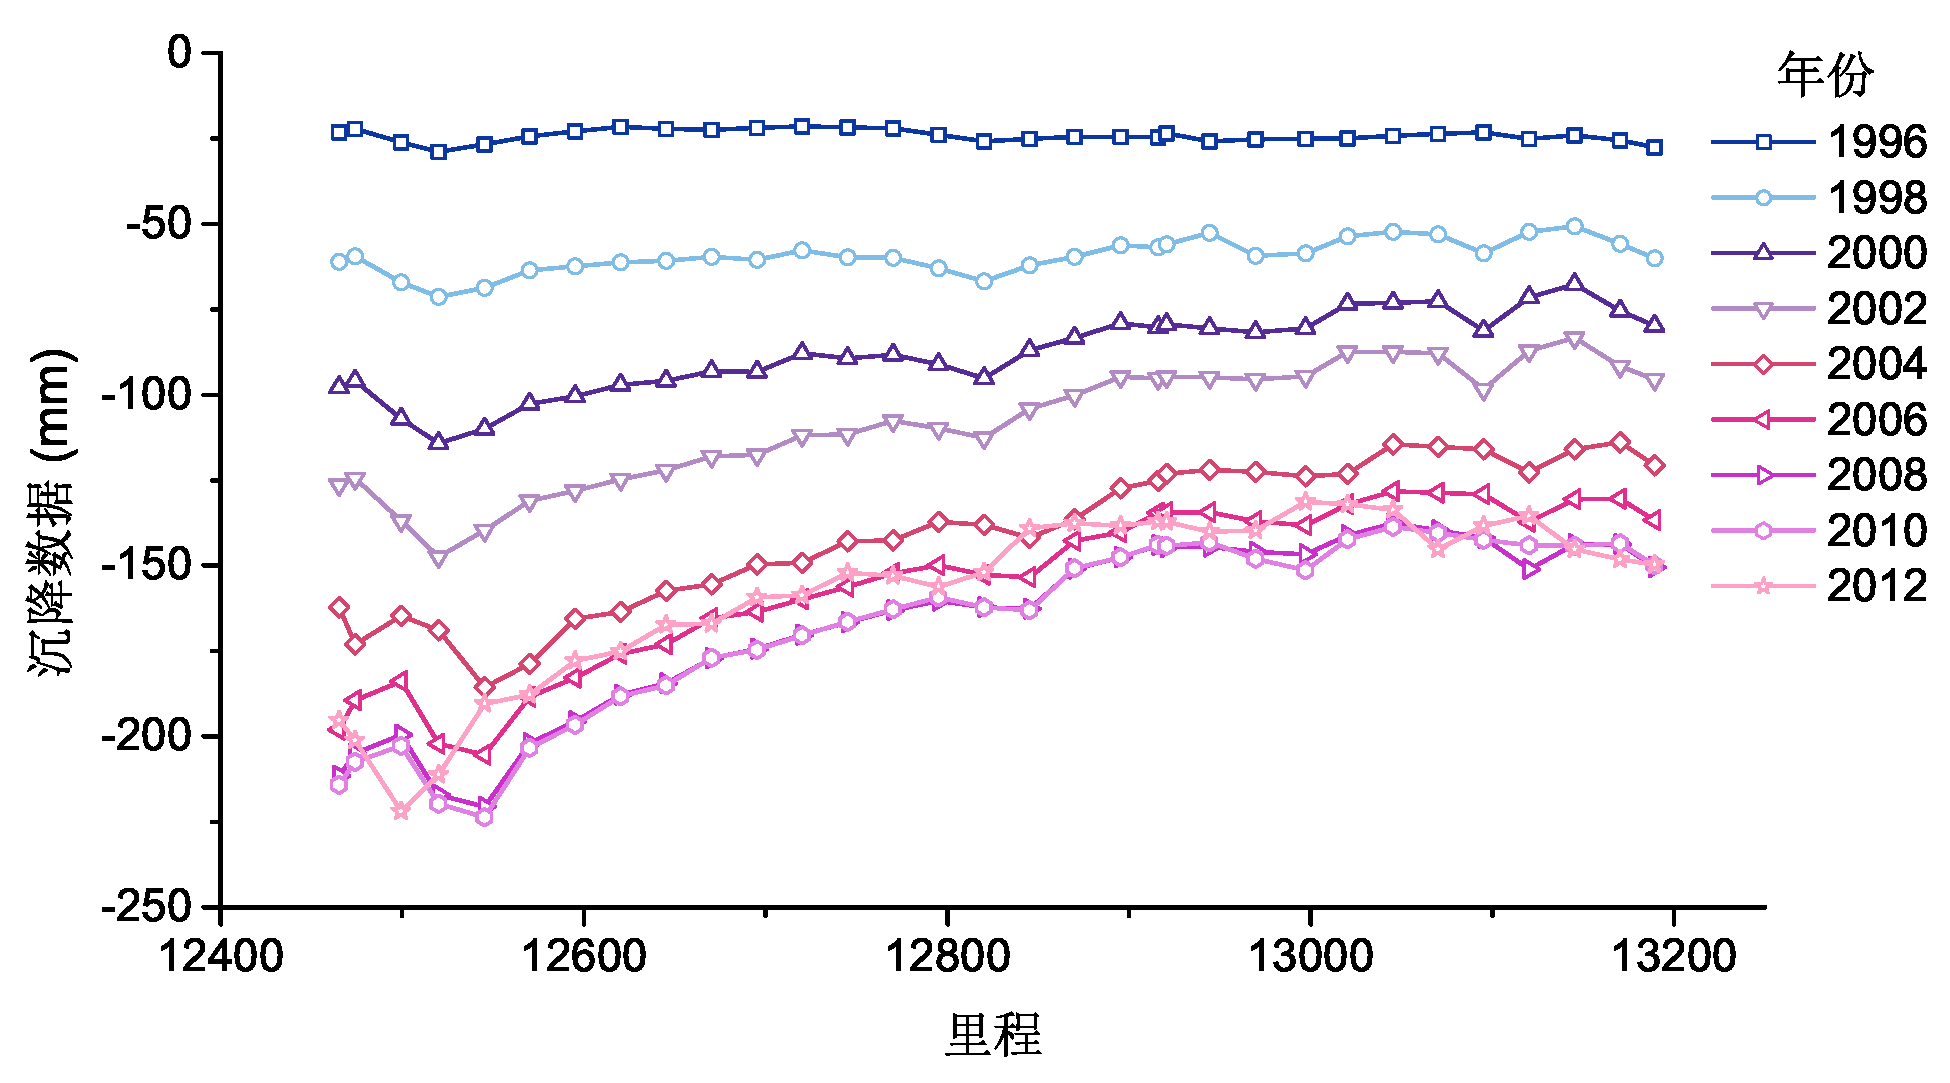
\includegraphics[width=1.0\textwidth]{chap3/sett-history.eps} \\ 
        (a)~区间不同年份沉降 \\
        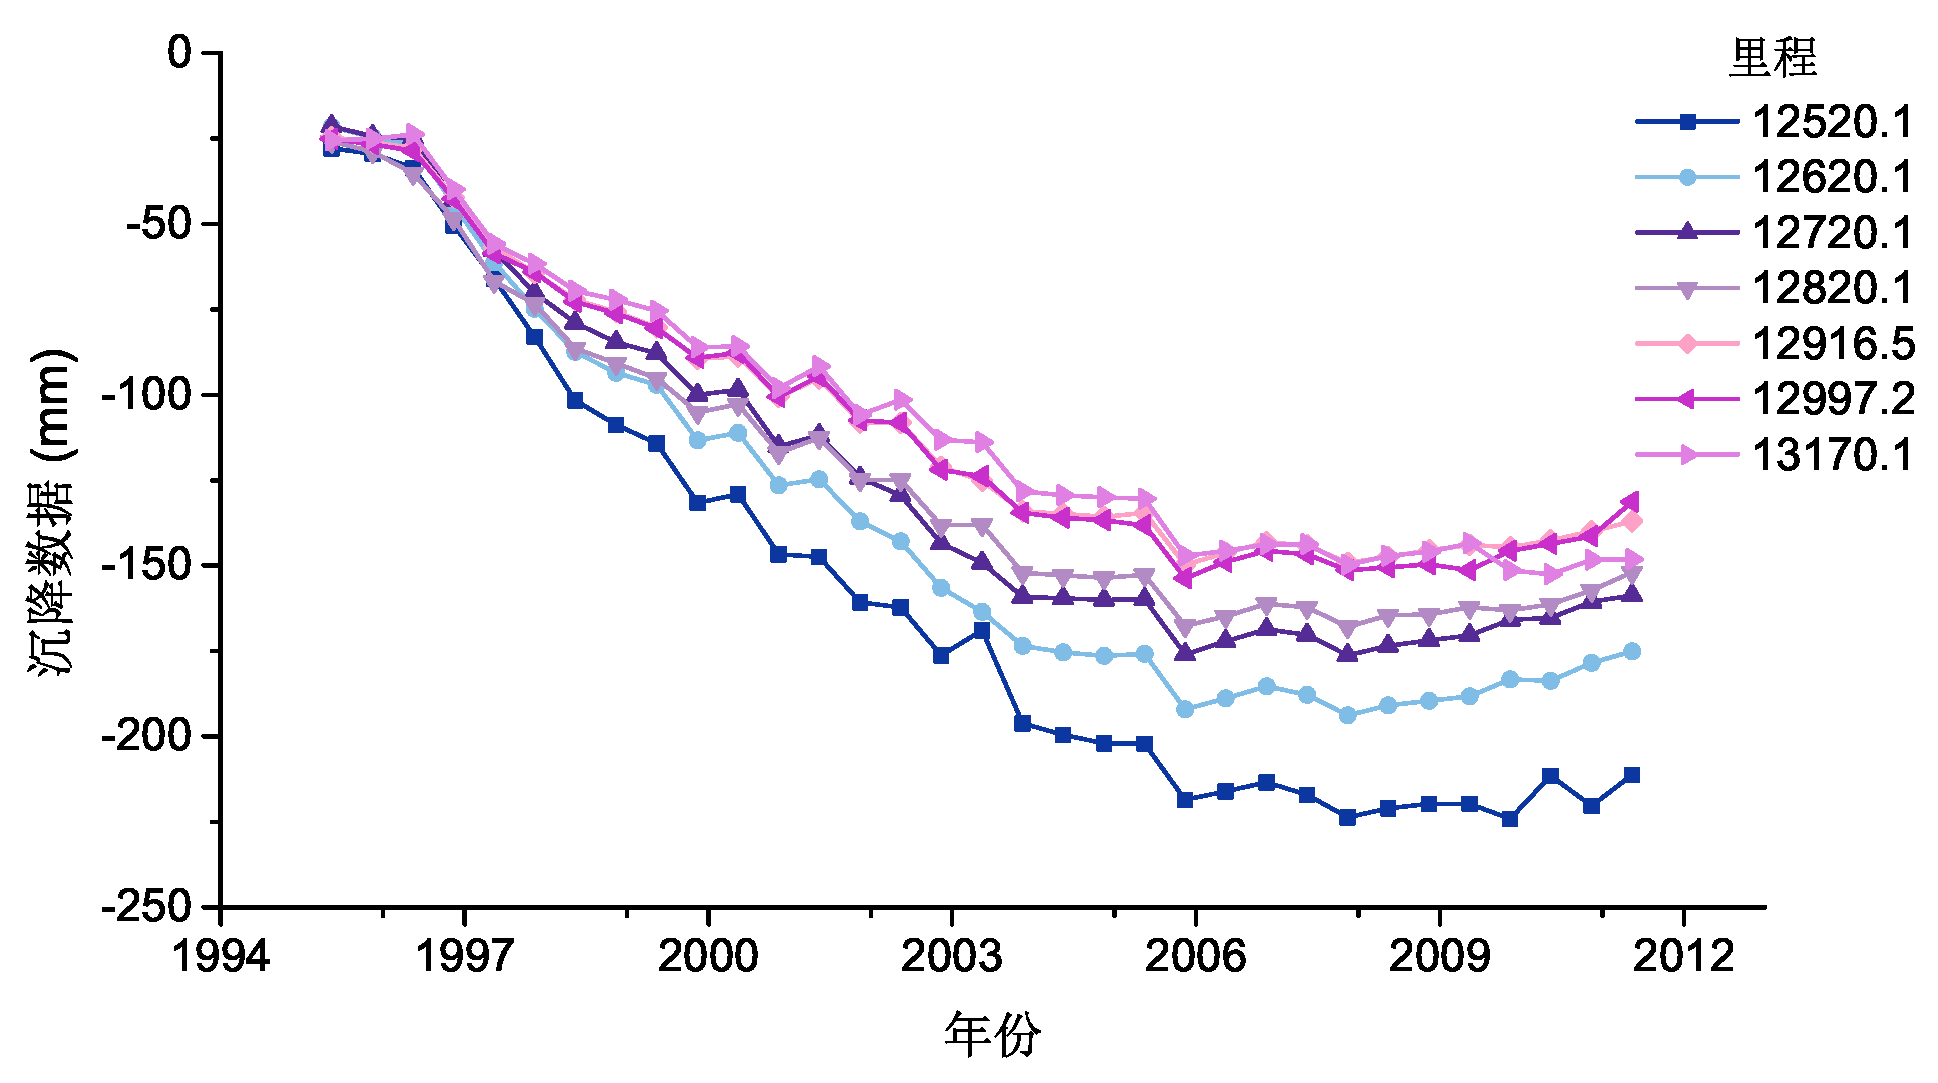
\includegraphics[width=1.0\textwidth]{chap3/sett-history2.eps} \\ 
        (b)~区间不同里程沉降 \\
    \end{tabular}
    \caption{地铁1号线新闸路-汉中路区间历史沉降} 
    \label{fig:地铁1号线新闸路-汉中路区间历史沉降} 
\end{figure}

%%%%%%%%%%%%%%%%%%%%%%%%%%%%%%%%%%%%%%%%%%%%%%%%%%%%%%%%%%%%%%%%%%%
\section{数据准备与处理}

%+++++++++++++++++++++++++++++++++++++++++++++++++++++++++++++++++%
\subsection{数据准备}

第~\ref{chap:tsi}~章采用沉降、收敛、渗漏水、裂缝和剥落评估隧道服役性能,对服役性能的预测即研究各个指标的退化模型。性能退化需建立在历年连续监测数据基础上,目前上海地铁对上述指标数据的采集情况如下:沉降数据从隧道建成开始,每年固定采集两次,如地铁1号线、2号线和4号线分别从1995年、1999年和2005年至今均有采集沉降数据;收敛数据在一开始并不作为日常监测的项目,随着近年对隧道横向变形的关注,这一指标才纳入监测范围,截止到2015年为止,地铁全线只在2011年、2012年和2014年进行过收敛数据的采集;对于病害数据,由于运营隧道里程长,人工检查速度慢,病害数据也只有在2011年和2012年进行过全线的检查,但随着病害采集车、无线传感、图像识别等技术的成熟,采集数据将会越来越多。

鉴于上述情况,本文只采用沉降数据作为研究对象,介绍预测方法原理及其应用,方法对于其他指标同样适用。以地铁1号线新闸路至汉中路区间为例,其历史沉降数据如图~\ref{fig:地铁1号线新闸路-汉中路区间历史沉降}~所示,整体来说,隧道的沉降曲线为两边高,中间低的形状(图~\ref{fig:地铁1号线新闸路-汉中路区间历史沉降}a),并且在隧道建成初期沉降速率快,随着运营年份的增加,沉降趋于稳定(图~\ref{fig:地铁1号线新闸路-汉中路区间历史沉降}b)。


%+++++++++++++++++++++++++++++++++++++++++++++++++++++++++++++++++%
\subsection{异常数据与缺失数据}

由于监测设备失灵、故障或人为失误、遗漏等原因,造成采集数据异常或者缺失,在作数据分析之前应对异常数据和缺失数据进行处理。异常数据一般可采用箱形图(Box-WhiskerPlot)进行处理,箱形图主要包含六个数据节点,分别为上边缘、上四分位数Q3、中位数、下四分位数Q1、下边缘和异常值,定义四分位距IQR=Q3-Q1,将Q3+1.5IQR和Q1-1.5IQR位置定义为异常值截断点,称其为内限,处于内限以外位置的点表示的数据可归为异常值。图~\ref{fig:地铁1号线新闸路-汉中路区间部分沉降箱形图}~所示为地铁1号线新闸路-汉中路区间部分沉降数据箱形图,从图中可知1996年4月和1998年4月采集的数据存在异常值,可将该数据删除后采用缺失数据处理方法补全。

\begin{figure}[htb!]
    \centering
    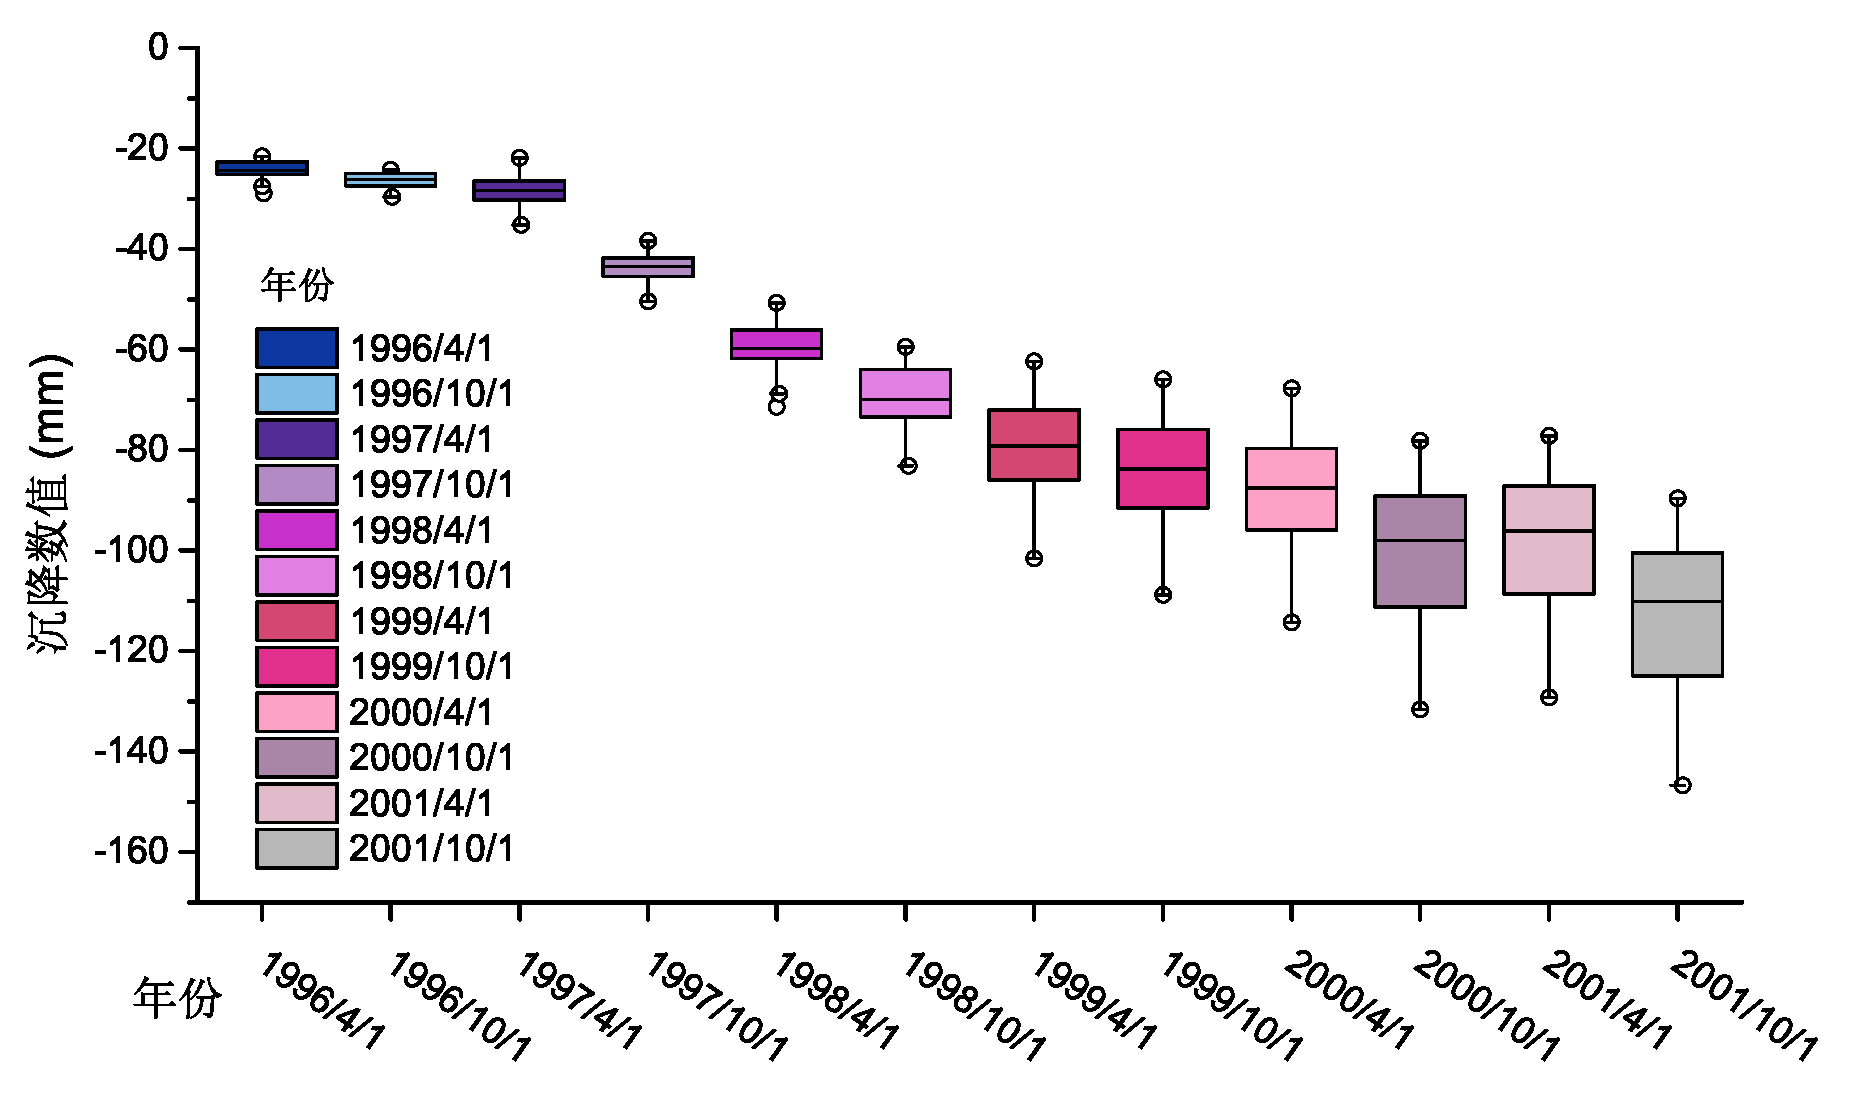
\includegraphics[width=1.0\textwidth]{chap3/boxplot.eps}
    \caption{地铁1号线新闸路-汉中路区间部分沉降箱形图}
    \label{fig:地铁1号线新闸路-汉中路区间部分沉降箱形图}
\end{figure}

常见的缺失数据处理方法有个案剔除法、均值替换法、回归替换法等,对于沉降数据的拟合可采用多项式、指数曲线、多段曲线、样条曲线等拟合,叶耀东(\citeyear{叶耀东2007软土地区运营地铁盾构隧道结构变形及健康诊断方法研究})提出三次均匀B样条曲线拟合实际隧道沉降,拟合方程为
\begin{equation}
    P(u)=\sum\limits_{i=0}^{n}{{{P}_{i}}{{N}_{i,k}}(u)}
\end{equation}
式中:${{P}_{i}}(i=0,1,\cdots ,n)$为沉降点,又称为德布尔点;${{N}_{i,k}}(u)(i=0,1,\cdots ,n)$称为$k$次规范B样条基函数。

本文采用三次样条曲线拟合的结果插值缺失数据较少的情况,在缺失数据较多时,上述方法的误差较大,则采用临近数据均值的方法插值,即取相邻里程的两个监测点,以及过去和未来一次的监测数据求和平均替代缺失数据。


%%%%%%%%%%%%%%%%%%%%%%%%%%%%%%%%%%%%%%%%%%%%%%%%%%%%%%%%%%%%%%%%%%%
\section{自回归与滑动平均时间序列模型}

%+++++++++++++++++++++++++++++++++++++++++++++++++++++++++++++++++%
\subsection{基本原理}

最出名的时间序列模型是由Box和Jenkins(\citeyear{box2015time})于1976年提出的自回归滑动平均时间序列(Autoregressive-Moving Average,ARMA),本节先简单介绍该模型的基本原理(EViews,\citeyear{noble2011eviews};潘红宇,\citeyear{cryer2011时间序列分析及应用})。

\subsubsection{自回归AR模型}

自回归模型就是用自身做回归变量,对于$p$阶自回归序列$\left\{ {{Y}_{t}} \right\}$满足方程:
\begin{align}
  \label{equ:AR1}
  & {{Y}_{t}}={{\rho }_{1}}{{Y}_{t-1}}+{{\rho }_{2}}{{Y}_{t-2}}+\cdots +{{\rho }_{p}}{{Y}_{t-p}}+{{\varepsilon }_{t}} \\ 
 & \quad =\sum\limits_{j=1}^{p}{{{\rho }_{j}}{{Y}_{t-j}}}+{{\varepsilon }_{t}} \nonumber
\end{align}
式中:${\varepsilon }_{t}$为新息项,包括了序列在$t$其无法用历史数据来解释的新新息,且${\varepsilon }_{t}$独立于${{Y}_{t-1}},{{Y}_{t-2}},{{Y}_{t-3}}\cdots $;${\rho }_{j}$为当前数据与历史数据的依赖关系系数。该式假设大于$p$阶滞后数据与当前数据没有关系。

为方便后续讨论,定义滞后算子$L$为
\begin{equation}
	\label{equ:lagL}
	{{L}^{k}}{{Y}_{t}}={{Y}_{t-k}}
\end{equation}
则式~\ref{equ:AR1}~可重写为
\begin{align}
  & {{Y}_{t}}=\sum\limits_{j=1}^{p}{{{\rho }_{j}}{{L}^{j}}{{Y}_{t}}}+{{\varepsilon }_{t}} \\ 
  \label{equ:lagL2}
 & \quad \rho (L){{Y}_{t}}={{\varepsilon }_{t}}
\end{align}
其中
\begin{equation}
	\label{equ:AR3}
	\rho (L)=1-\sum\limits_{j=1}^{p}{{{\rho }_{j}}{{L}^{j}}}
\end{equation}
为滞后算子多项式,如果该时间序列均值不为0,则设$t$时刻时间序列均值为${{\mu }_{t}}$,则式~\ref{equ:lagL2}~可以写成
\begin{equation}
	\rho (L)({{Y}_{t}}-{{\mu }_{t}})={{\varepsilon }_{t}}
\end{equation}
对于$p$阶AR模型,假设均值${{\mu }_{t}}$为外部变量${X'}_{t}$的线性组合,即${{\mu }_{t}}={{{X}'}_{t}}\beta $,则$p$阶的AR(p)模型最终如下:
\begin{gather}
  	{{Y}_{t}}={{{{X}'}}_{t}}\beta +{{u}_{t}} \\ 
 	{{u}_{t}}={{\rho }_{1}}{{u}_{t-1}}+{{\rho }_{2}}{{u}_{t-2}}+\cdots +{{\rho }_{p}}{{u}_{t-p}}+{{\varepsilon }_{t}} \\ 
 	{{Y}_{t}}={{{{X}'}}_{t}}\beta +\sum\limits_{j=1}^{p}{{{\rho }_{j}}({{Y}_{t-j}}-{{{{X}'}}_{t-j}}\beta )+}{{\varepsilon }_{t}} \\ 
 	\left( 1-\sum\limits_{j=1}^{p}{{{\rho }_{j}}{{L}^{j}}} \right)({{Y}_{t}}-{{{{X}'}}_{t}}\beta )={{\varepsilon }_{t}} 
\end{gather}

\subsubsection{滑动平均MA模型}

滑动平均MA模型的$q$阶形式为
\begin{align}
  & {{Y}_{t}}={{\varepsilon }_{t}}+{{\theta }_{1}}{{\varepsilon }_{t-1}}+{{\theta }_{2}}{{\varepsilon }_{t-2}}+\cdots +{{\theta }_{q}}{{\varepsilon }_{t-q}} \nonumber \\ 
 & \quad ={{\varepsilon }_{t}}+\sum\limits_{j=1}^{q}{{{\theta }_{j}}{{\varepsilon }_{t-j}}} \\ 
 & \quad =\theta (L){{\varepsilon }_{t}} \nonumber
\end{align}
式中:${\theta }_{j}$为新息项的系数,且
\begin{equation}
	\theta (L)=1+\sum\limits_{j=1}^{q}{{{\theta }_{j}}{{L}^{j}}}
\end{equation}
是滑动平均模型的${\theta }$多项式,代表MA模型的特性,若MA模型的均值不为0,则可记
\begin{equation}
	\label{equ:MA1}
	{{Y}_{t}}-\mu =\theta (L){{\varepsilon }_{t}}
\end{equation}

\subsubsection{自回归滑动平均ARMA模型}

自回归滑动平均模型是由AR模型和MA模型组合得到,结合式~\ref{equ:AR3}~和式~\ref{equ:MA1}~可得
\begin{equation}
	\rho (L)({{Y}_{t}}-{{\mu }_{t}})=\theta (L){{\varepsilon }_{t}}
\end{equation}
对于$p$阶AR模型和$q$阶MA模型的组合命名为ARMA(p,q)。最简单的ARMA模型由1阶AR和1阶MA组成的ARMA(1,1),如下:
\begin{gather}
 	{{Y}_{t}}={{{{X}'}}_{t}}\beta +{{u}_{t}} \\ 
	{{u}_{t}}=\rho {{u}_{t-1}}+{{\varepsilon }_{t}}+\theta {{\varepsilon }_{t-1}}
\end{gather}
式中:$\rho$为一阶AR模型参数;$\theta$为一阶MA模型参数。代入后ARMA(1,1)模型可写为
\begin{align}
  & {{Y}_{t}}={{{{X}'}}_{t}}\beta +\rho {{u}_{t-1}}+{{\varepsilon }_{t}}+\theta {{\varepsilon }_{t-1}} \\ 
 & ={{{{X}'}}_{t}}\beta +\rho ({{Y}_{t-1}}-{{{{X}'}}_{t-1}}\beta )+{{\varepsilon }_{t}}+\theta {{\varepsilon }_{t-1}}
\end{align}
采用滞后算子$L$可简写为
\begin{equation}
	(1-\rho L)({{Y}_{t}}-{{{X}'}_{t}}\beta )=(1+\theta L){{\varepsilon }_{t}}
\end{equation}

%+++++++++++++++++++++++++++++++++++++++++++++++++++++++++++++++++%
\subsection{模型建立}
\label{chap:armamodelbuilding}

上述介绍的AR、MA和ARMA模型不存在哪个模型是最优的,它们分别描述了时间序列的自然属性,在建立时间序列模型时需选择合适的模型和滞后阶数。时间序列模型要求分析的序列是平稳的,但在实际中大部分的序列都是非平稳的,需将非平稳时间序列转化成平稳时间序列。一般的序列通过一阶差分(式~\ref{equ:diff1}~)或二阶差分(式~\ref{equ:diff2}~)可转换成平稳序列(Hamilton,\citeyear{hamilton1994time})。
\begin{gather}
	\label{equ:diff1}
	\nabla {{Y}_{t}}={{Y}_{t}}-{{Y}_{t-1}} \\ 
	\label{equ:diff2}
	{{\nabla }^{2}}{{Y}_{t}}=\nabla \nabla {{Y}_{t}}=({{Y}_{t}}-{{Y}_{t-1}})-({{Y}_{t-1}}-{{Y}_{t-2}}) 
\end{gather}
定量化的判断序列是否平稳可采用Dickey-Fuller单位根进行验证检验(Dickey和Fuller,\citeyear{dickey1979distribution})。

对于观测到的时间序列${{Y}_{1}},{{Y}_{2}},\cdots ,{{Y}_{n}}$,定义时间序列的自相关函数(Autocorrelation Function,ACF)为
\begin{equation}
	{{r}_{k}}=\frac{\sum\limits_{t=k+1}^{n}{({{Y}_{t}}-\bar{Y})({{Y}_{t-k}}-\bar{Y})}}{\sum\limits_{t=1}^{n}{{{({{Y}_{t}}-\bar{Y})}^{2}}}},k=1,2\cdots 
\end{equation}
定义消除中间介入变量${{Y}_{t-1}},{{Y}_{t-2}},{{Y}_{t-3}},\cdots ,{{Y}_{t-k+1}}$的影响后$Y_t$和$Y_{t-k}$的相关系数函数为偏相关系数(Partial Autocorrelation Function,PACF),即
\begin{equation}
	{{\rho }_{kk}}=Corr({{Y}_{t}},{{Y}_{t-k}}|{{Y}_{t-1}},{{Y}_{t-2}},\cdots ,{{Y}_{t-k+1}})
\end{equation}

通过观察自相关图与偏相关图可确定ARMA(p,q)模型的具体形式,有两个相关概念:(1)拖尾:指的是ACF或者PACF随滞后阶数呈几何衰减;(2)截尾:指的是ACF或者PACF在某一阶不为0,之后突然接近或者等于0。

AR(p)模型,从自相关函数ACF来看,在自回归方程的基础上可以很简单构造ACF,自相关系数等于${{\rho }^{k}}$(${\rho }$为自回归系数,$k$为滞后数),对于平稳时间序列,$\left| \rho  \right|<1$,所以当${\rho }>0$时,ACF呈现为指数式衰减至0.当${\rho }<0$时,ACF则正负交替呈指数衰减至0,整体表现则是正弦式衰减;从偏相关函数PACF来看,其与自回归方程的形式完全一样,只是自回归方程只有滞后$p$期,而PACF则有更多的滞后项。于是乎,当$k\le p$,偏相关系数不等于0,当$k>p$,偏相关系数等于0,明显呈现出截尾现象。

MA(q)模型,从自相关函数ACF来看,在移动平均方程的基础上也可以很简单地构造自相关系数,这时候的自相关函数为分段函数,当$k\le q$,偏相关系数不等于0,当$k>q$,偏相关系数等于0,明显呈现出截尾现象;从偏相关函数PACF来看,任何一个可逆的MA(q)过程都可以转换成一个无限阶、系数按几何衰减的AR过程(将白噪声替换为序列的滞后形式即可),呈现拖尾现象。与AR(p)不同的是,当$\theta >0$($\theta$为移动平均系数)时,PACF呈现为交替式正弦衰减。当$\theta <0$时,PACF则呈指数衰减至0。ARMA(p,q)模型则是两者的结合,总结如表~\ref{tab:armaarma}~所示。

\begin{table}[htb!]
  \centering
  \caption{AR、MA、ARMA模型识别}
    \begin{tabular}{?m{11em}<{\centering}"m{9em}<{\centering}"m{9em}<{\centering}?}
    \thickhline
    模型定阶  & 自相关系数 & 偏相关系数 \bigstrut\\
    \thinhline
    AR(p)模型 & 拖尾    & p阶截尾 \bigstrut\\
    \thinhline
    MA(q)模型 & q阶截尾  & 拖尾 \bigstrut\\
    \thinhline
    ARMA(p,q)模型 & 拖尾    & 拖尾 \bigstrut\\
    \thickhline
    \end{tabular}%
  \label{tab:armaarma}%
\end{table}%

除了根据拖尾和截尾的属性,还可以采用AIC(Akaike Information Criterion)(Akaike,\citeyear{akaike2011akaike})和BIC(Schwarz Criterion)(Schwarz,\citeyear{schwarz1978estimating})准则进行模型识别。在确定了模型阶数后,可采用矩估计、最小二乘估计和极大似然估计等方法进行参数估计。

%+++++++++++++++++++++++++++++++++++++++++++++++++++++++++++++++++%
\subsection{模型验证}

时间序列模型的验证可验证模型残差$\left\{ {{\varepsilon }_{t}} \right\}$是否为白噪声,若残差不是白噪声,则说明残差中的信息并未完全提取,应考虑重新选定模型。

白噪声验证可通过${{\chi }^{2}}$检验验证。${{\chi }^{2}}$是一种简单又高效的检验方法,其证明$m$个独立的$N(0,1)$分布的随机变量的平方和为自由度为$m$的${{\chi }^{2}}$分布,残差的自相关函数为
\begin{equation}
	{{\gamma }_{k}}(\varepsilon )=\frac{\sum\limits_{t=1}^{N-k}{{{\varepsilon }_{t}}{{\varepsilon }_{t+k}}}}{\sum{\varepsilon _{t}^{2}}}
\end{equation}
当$n\to \infty$,$\sqrt{N}{{\gamma }_{k}}(\varepsilon )\tilde{\ }N(0,1)(k=1,2,\cdots ,m)$。

原假设:残差序列之间相互独立。则残差${{\chi }^{2}}$统计量
\begin{equation}
	{{Q}_{m}}=\sum\limits_{k=1}^{m}{{{\left[ \sqrt{N}{{\gamma }_{k}}(\varepsilon ) \right]}^{2}}=n\sum\limits_{k=1}^{m}{\gamma _{k}^{2}(\varepsilon )}}
\end{equation}
式中:$n$为观测数据个数;$m$为最大的时滞。

在显著性水平$\alpha $下,记${{\chi }^{2}}$为$\chi _{\alpha }^{2}$。比较${{\chi }^{2}}$与$Q_m$的大小,如果${{Q}_{m}}\le \chi _{\alpha }^{2}$,则接受原假设,即残差为白噪声;反之,拒绝原假设,即残差不是白噪声。


%+++++++++++++++++++++++++++++++++++++++++++++++++++++++++++++++++%
\subsection{盾构隧道ARMA模型建模}
\label{chap:armatunnel}

根据上述时间序列理论,建立时间序列模型大致可以分为稳定性判断、模型识别和模型验证几个步骤,如图~\ref{fig:ARMA时间序列模型建模流程图}~所示。

\begin{figure}[htb!]
    \centering
    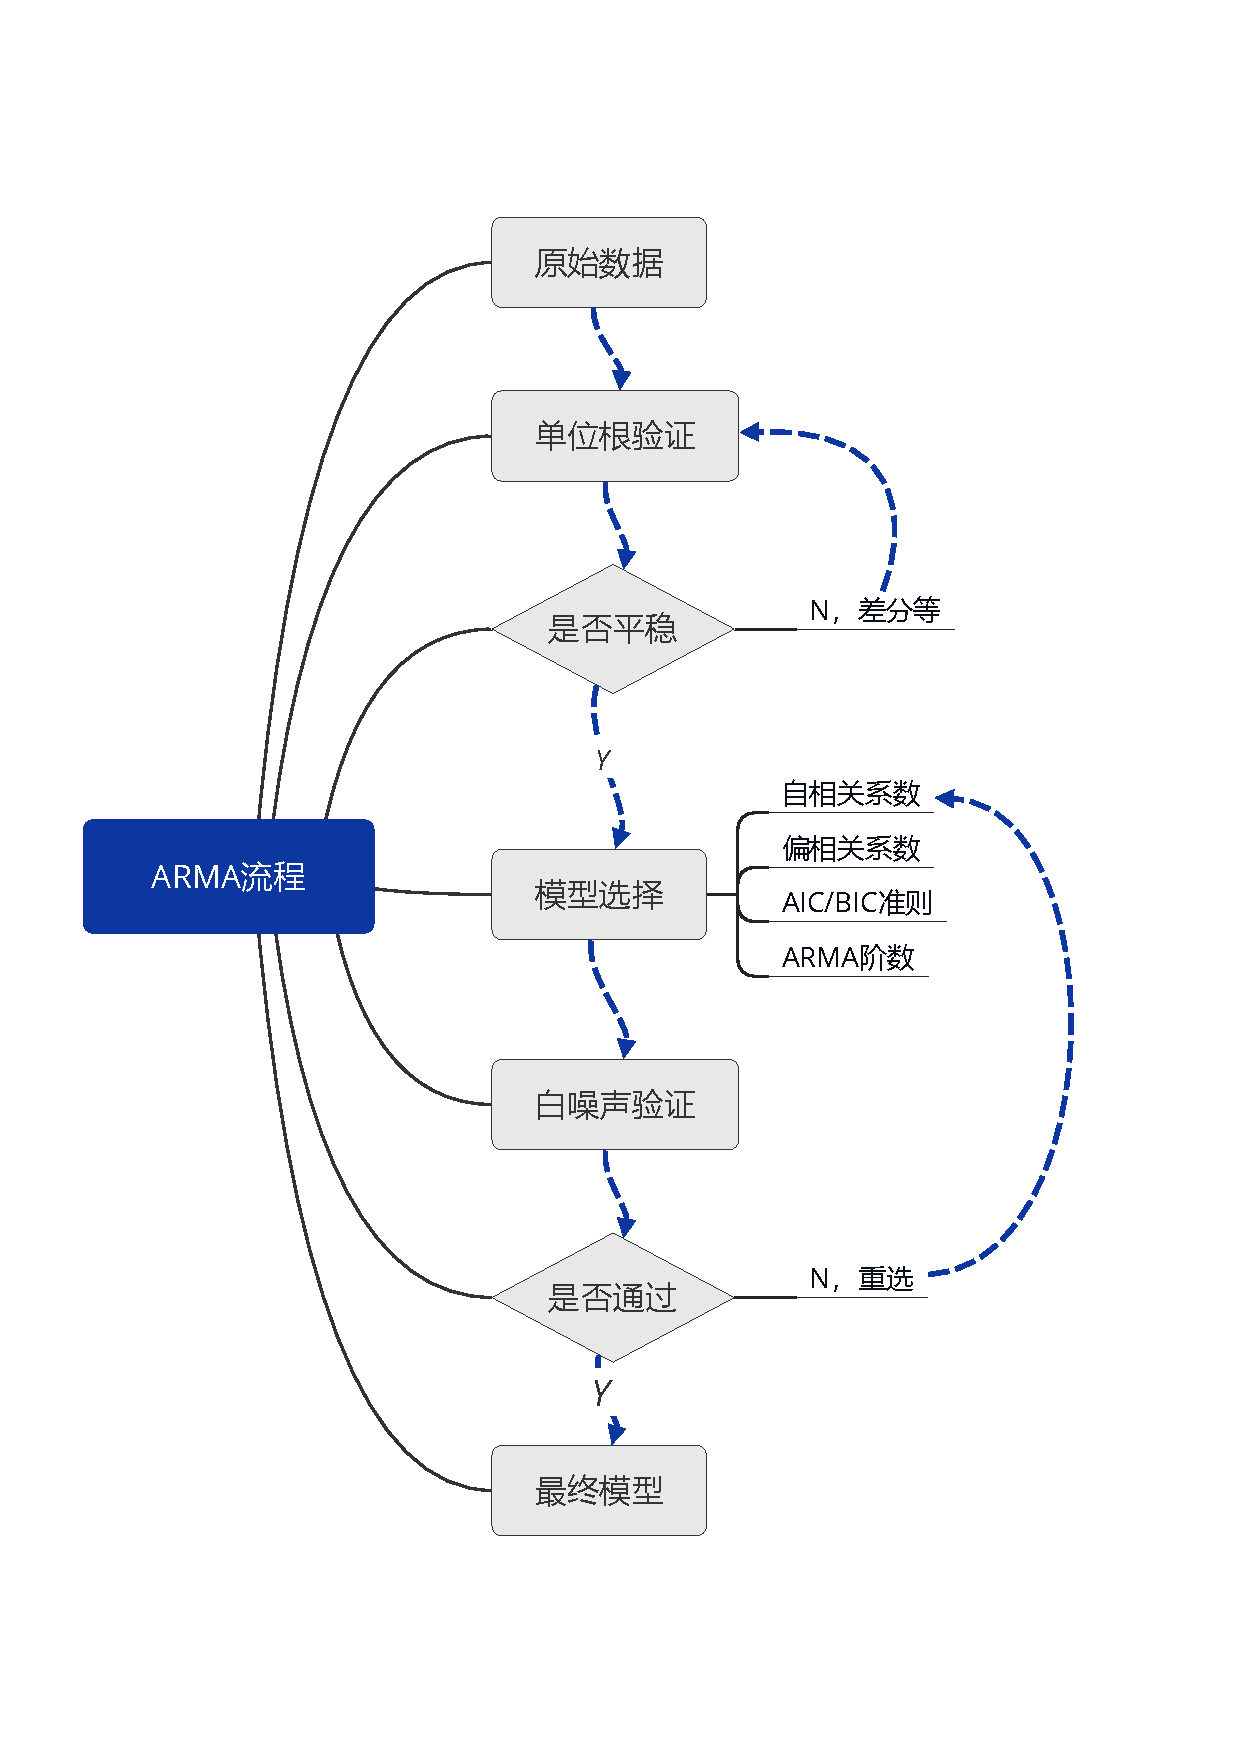
\includegraphics[width=0.55\textwidth]{chap3/time-series-process.pdf}
    \caption{ARMA时间序列模型建模流程图}
    \label{fig:ARMA时间序列模型建模流程图}
\end{figure}

\subsubsection{稳定性判断}

以上海地铁1号新闸路至汉中路下行线,里程为12916.05的沉降监测点为例,介绍沉降ARMA模型建立。首先根据原始数据计算自相关和偏相关图,如表~\ref{tab:原始沉降数据的自相关与偏相关系数}~所示。由自相关图可看到,自相关系数递减缓慢,并且在时滞为10时候,仍大于两倍标准差范围,可以判断沉降数据存在趋势。另一方面,观察图~\ref{fig:地铁1号线新闸路-汉中路区间历史沉降}b~可以看出数据存在明显的趋势,在一开始数据增加速度较快,后期则逐渐减缓,且存在一定的波动。

可考虑采用线性回归或者差分的方法将数据转化为平稳数据。对于沉降数据,随着隧道运营时间增长,沉降逐渐趋于稳定,甚至沉降还会有回弹,很难用某一回归模型进行拟合,而且回归模型对于未来的数据趋势拟合也不一定很好。故本文采用差分的方法进行数据平稳化处理。根据~\ref{chap:armamodelbuilding}~小节采用单位根ADF检验判断序列是否存在单位根,若ADF的统计量比置信区间的临界值大,则不能拒绝序列存在单位根的假设,即序列是非平稳的。一般取置信区间为0.5\%。计算结果如表~\ref{tab:沉降数据差分稳定性分析}~所示,原始数据的单位根t统计量为-3.882999,显著性水平为0.0058,不足以拒绝原始数据存在单位根的假设。一阶差分的单位根t统计量为-2.268996,显著性水平为0.1880,一阶差分后的序列仍然不是平稳的。二阶差分的单位根t统计量为-7.312877,足以拒绝原假设,即沉降数据经过二阶差分后为平稳数据。但是有一点需要注意,虽然差分运算可以将数据平稳化,但差分后数据的物理意义可能存在难以解释的问题,如沉降数据的一阶差分为沉降速率,二阶差分则表示沉降加速度。

\begin{table}[htb!]
  \centering
  \caption{原始沉降数据的自相关与偏相关系数}
    \begin{tabular}{?c"m{8em}<{\centering}"m{8em}<{\centering}"c"c"c"c?}
    \thickhline
    阶数    & 自相关系数 & 偏相关系数 & AC    & PAC   & Q-Stat & Prob \bigstrut\\
    \thinhline
    1     & \multirow{12}[24]{*}{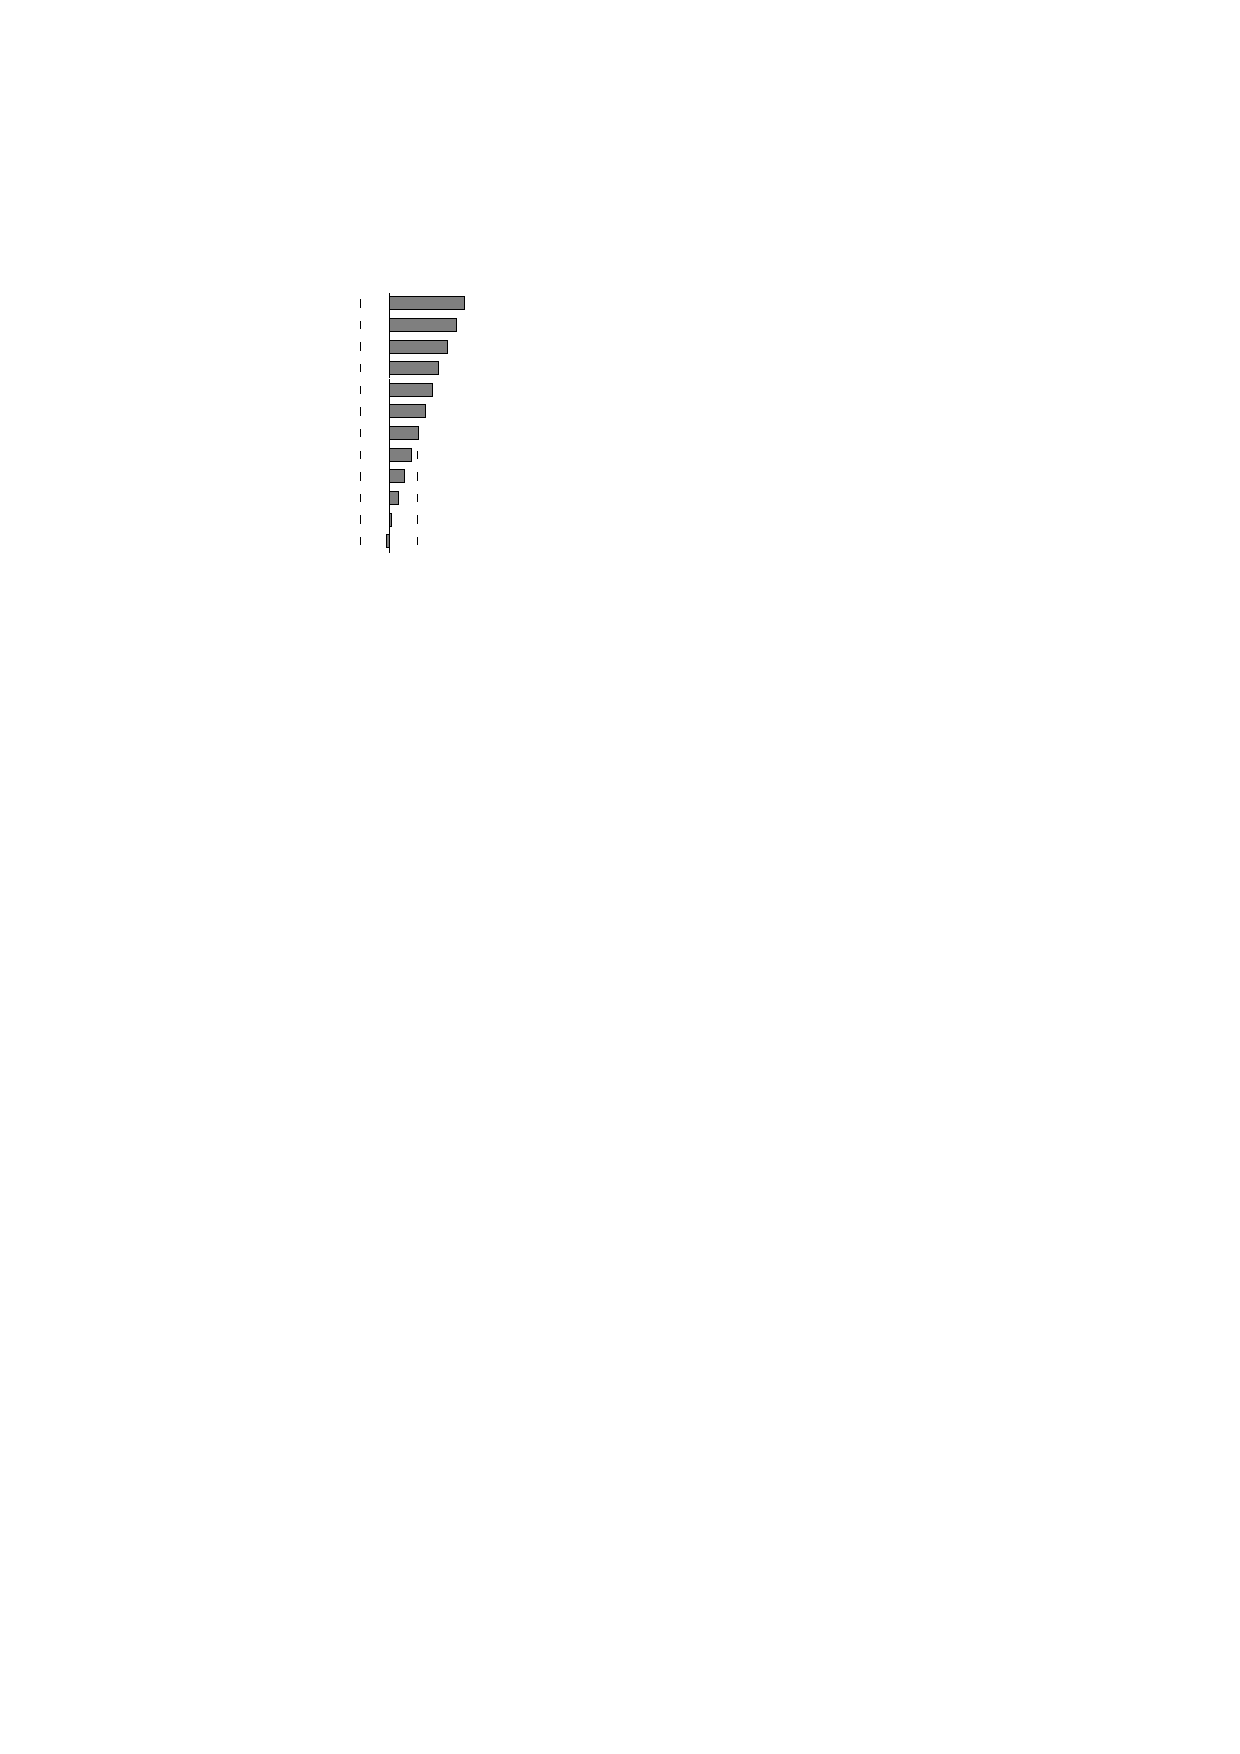
\includegraphics[width=8em,height=22.2em]{chap3/ACF1.pdf}} & \multirow{12}[24]{*}{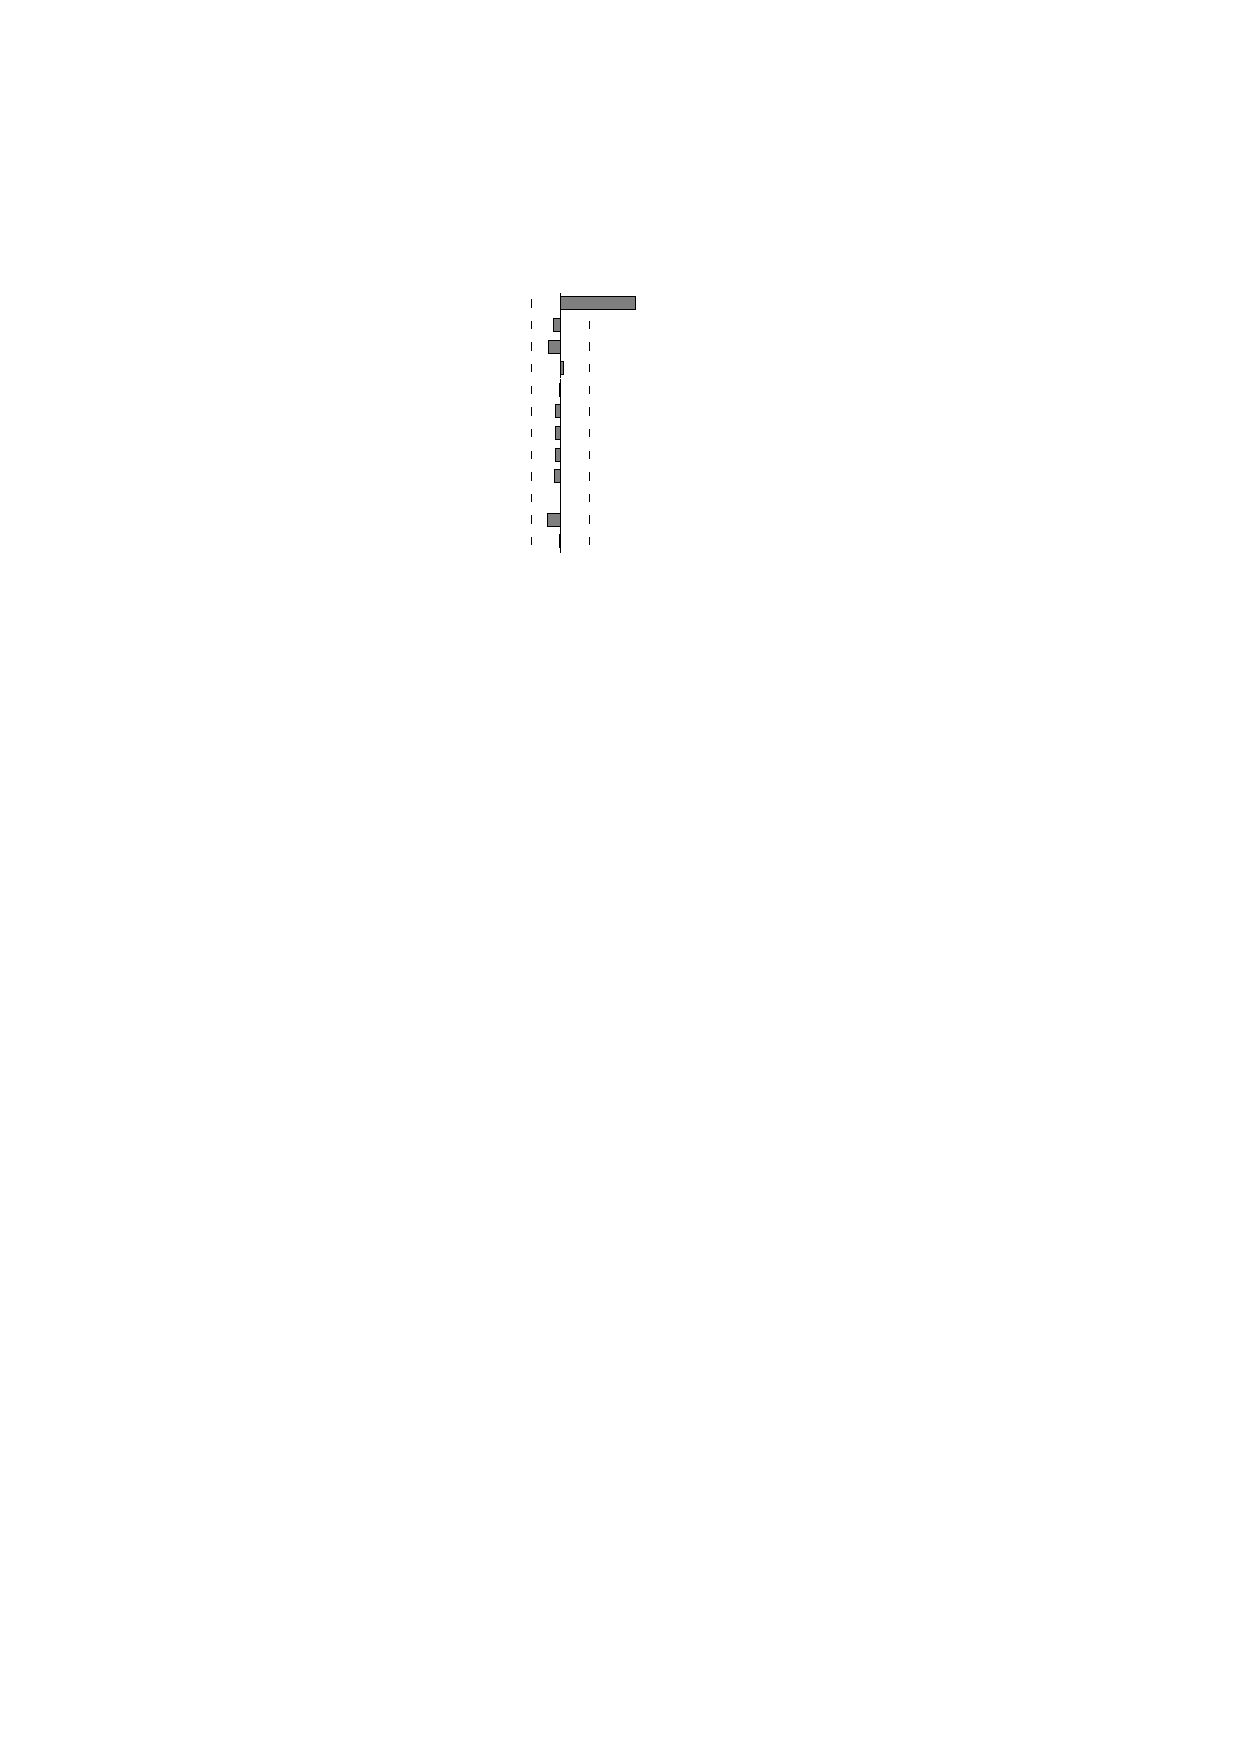
\includegraphics[width=8em,height=22.2em]{chap3/PACF1.pdf}} & 0.910  & 0.910  & 29.893  & 0.000  \bigstrut\\
\cline{1-1}\cline{4-7}    2     &       &       & 0.813  & -0.086  & 54.550  & 0.000  \bigstrut\\
\cline{1-1}\cline{4-7}    3     &       &       & 0.702  & -0.142  & 73.500  & 0.000  \bigstrut\\
\cline{1-1}\cline{4-7}    4     &       &       & 0.606  & 0.038  & 88.134  & 0.000  \bigstrut\\
\cline{1-1}\cline{4-7}    5     &       &       & 0.519  & -0.010  & 99.237  & 0.000  \bigstrut\\
\cline{1-1}\cline{4-7}    6     &       &       & 0.436  & -0.052  & 107.360  & 0.000  \bigstrut\\
\cline{1-1}\cline{4-7}    7     &       &       & 0.353  & -0.056  & 112.910  & 0.000  \bigstrut\\
\cline{1-1}\cline{4-7}    8     &       &       & 0.271  & -0.056  & 116.300  & 0.000  \bigstrut\\
\cline{1-1}\cline{4-7}    9     &       &       & 0.188  & -0.069  & 118.000  & 0.000  \bigstrut\\
\cline{1-1}\cline{4-7}    10    &       &       & 0.116  & 0.006  & 118.680  & 0.000  \bigstrut\\
\cline{1-1}\cline{4-7}    11    &       &       & 0.032  & -0.151  & 118.730  & 0.000  \bigstrut\\
\cline{1-1}\cline{4-7}    12    &       &       & -0.039  & -0.007  & 118.820  & 0.000  \bigstrut\\
    \thickhline
    \end{tabular}%
  \label{tab:原始沉降数据的自相关与偏相关系数}%
\end{table}%

\begin{table}[htb!]
  \centering
  \caption{沉降数据差分稳定性分析}
    \begin{tabular}{?m{8em}<{\centering}"m{12em}<{\centering}"m{7em}<{\centering}"c?}
    \thickhline
    \multicolumn{2}{?c"}{原始数据} & t统计量  & 显著性水平 \bigstrut\\
    \thinhline
    \multicolumn{2}{?c"}{Dickey-Fuller单位根} & -3.882999  & 0.0058  \bigstrut\\
    \thinhline
    \multirow{3}[6]{*}{检验的临界值} & 1\%显著性水平 & -3.661661  &  \bigstrut\\
\cline{2-4}          & 5\%显著性水平 & -2.960411  &  \bigstrut\\
\cline{2-4}          & 10\%显著性水平 & -2.619160  &  \bigstrut\\
    \thinhline
    \multicolumn{2}{?c"}{一阶差分} &       &  \bigstrut\\
    \thinhline
    \multicolumn{2}{?c"}{Dickey-Fuller单位根} & -2.268996  & 0.1880  \bigstrut\\
    \thinhline
    \multirow{3}[6]{*}{检验的临界值} & 1\%显著性水平 & -3.670170  &  \bigstrut\\
\cline{2-4}          & 5\%显著性水平 & -2.963972  &  \bigstrut\\
\cline{2-4}          & 10\%显著性水平 & -2.621007  &  \bigstrut\\
    \thinhline
    \multicolumn{2}{?c"}{二阶差分} &       &  \bigstrut\\
    \thinhline
    \multicolumn{2}{?c"}{Dickey-Fuller单位根} & -7.312877  & 0.0000  \bigstrut\\
    \thinhline
    \multirow{3}[6]{*}{检验的临界值} & 1\%显著性水平 & -3.689194  &  \bigstrut\\
\cline{2-4}          & 5\%显著性水平 & -2.971853  &  \bigstrut\\
\cline{2-4}          & 10\%显著性水平 & -2.625121  &  \bigstrut\\
    \thickhline
    \end{tabular}%
  \label{tab:沉降数据差分稳定性分析}%
\end{table}%

\subsubsection{模型识别}

确定二阶差分形式为稳定序列后,绘制沉降二阶差分的自相关和偏相关函数,如表~\ref{tab:沉降数据二阶差分的自相关与偏相关系数}~所示。由表中可知,在时滞大于4的时候,自回归系数大小落入两倍标准差范围内,在时滞大于3的时候,偏回归系数大小落入两倍标准差范围内,ACF和PACF均有拖尾的现象,可尝试ARMA(3,4)阶数以下的ARMA模型,如AR(1)、AR(2)、AR(3)、MA(1)、MA(2)、MA(3)、MA(4)、AR(1,1)、AR(1,2)、AR(1,3)等,根据~\ref{chap:armamodelbuilding}~小节理论,采用极大似然法对模型参数进行估计,计算参数的t检验值,如表~\ref{tab:不同ARMA模型的参数估计}~所示,并计算了各个模型的残差平方和、AIC和BIC值,如表~\ref{tab:不同ARMA模型的残差平方和AIC和BIM}~所示。

\begin{table}[htb!]
  \centering
  \caption{沉降数据二阶差分的自相关与偏相关系数}
    \begin{tabular}{?c"m{8em}<{\centering}"m{8em}<{\centering}"c"c"c"c?}
    \thickhline
    阶数    & 自相关系数 & 偏相关系数 & AC    & PAC   & Q-Stat & Prob \bigstrut\\
    \thinhline
    1     & \multirow{12}[24]{*}{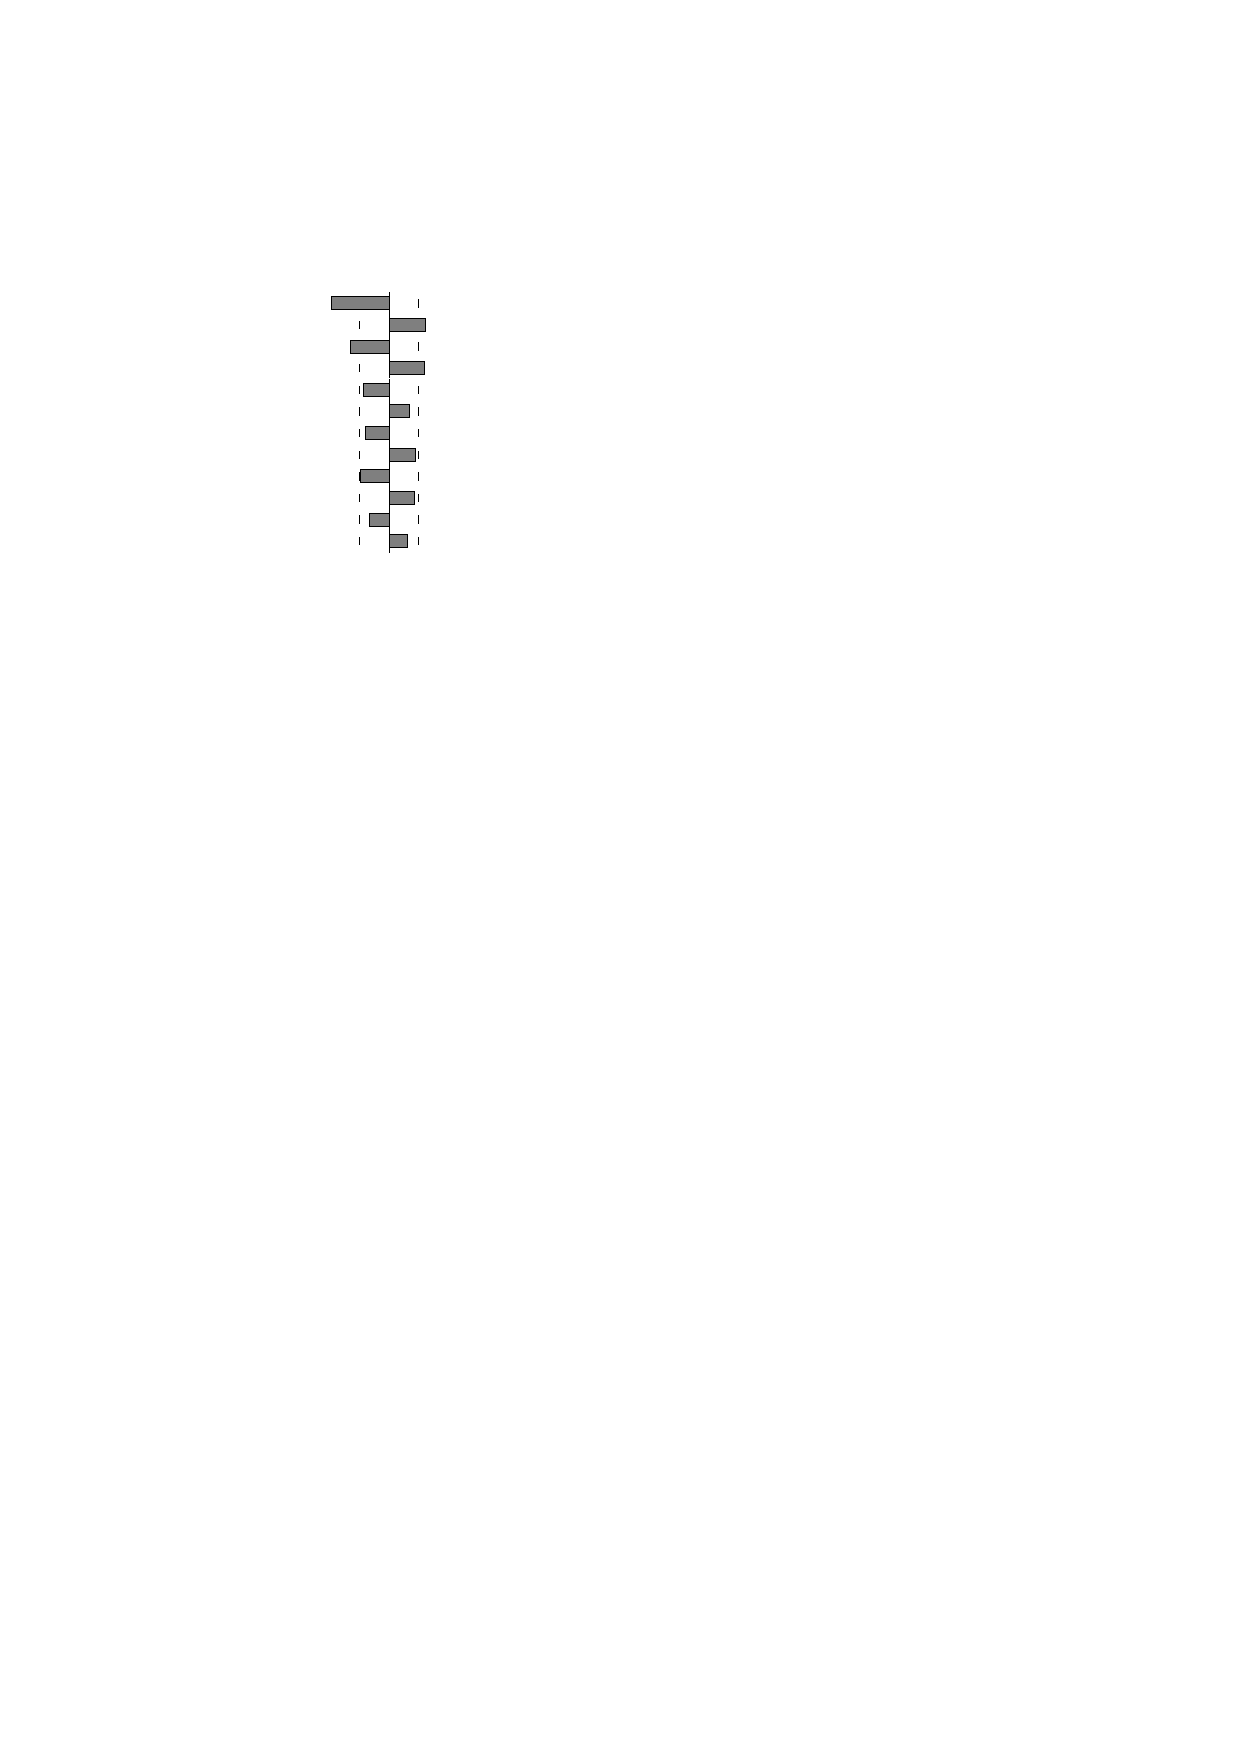
\includegraphics[width=8em,height=22.2em]{chap3/ACF2.pdf}} & \multirow{12}[24]{*}{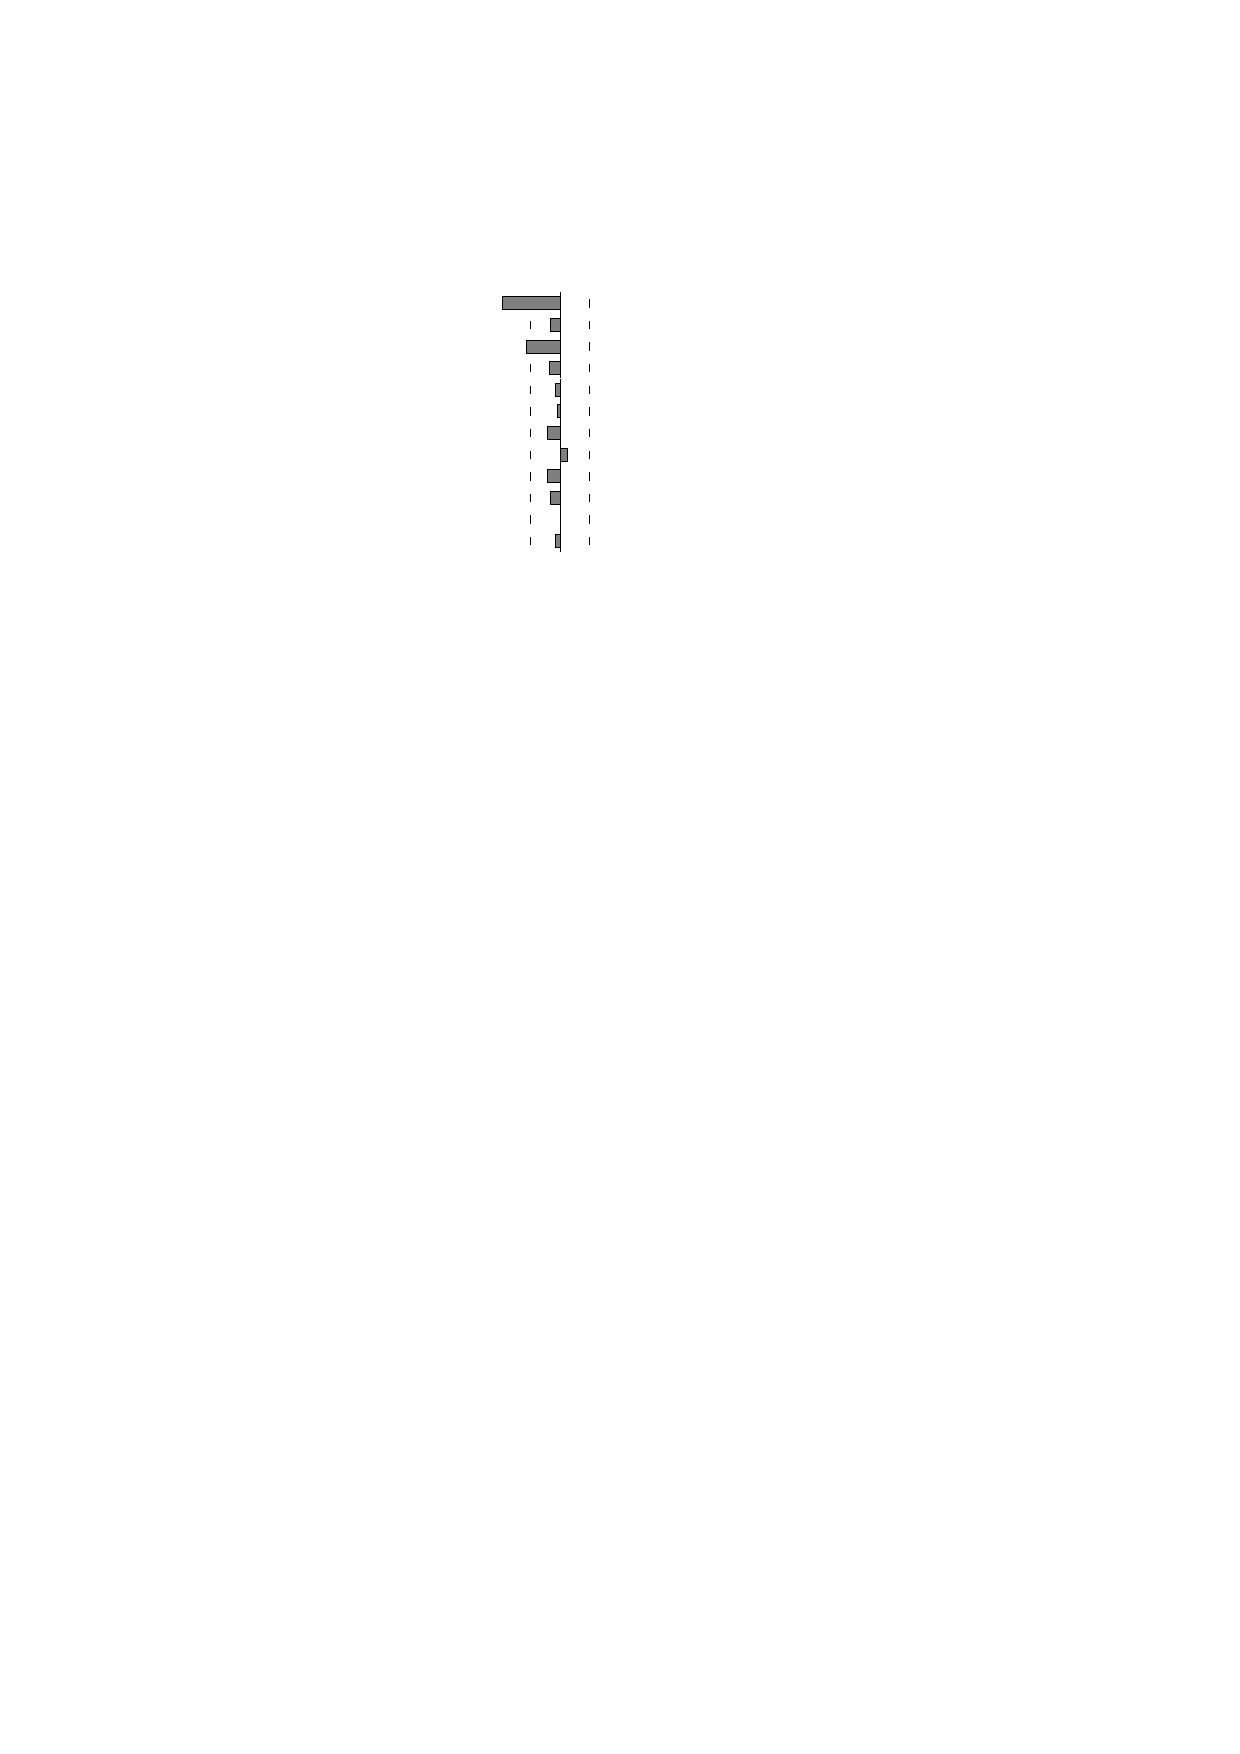
\includegraphics[width=8em,height=22.2em]{chap3/PACF2.pdf}} & -0.705  & -0.705  & 16.929  & 0.000  \bigstrut\\
\cline{1-1}\cline{4-7}    2     &       &       & 0.436  & -0.120  & 23.634  & 0.000  \bigstrut\\
\cline{1-1}\cline{4-7}    3     &       &       & -0.464  & -0.413  & 31.510  & 0.000  \bigstrut\\
\cline{1-1}\cline{4-7}    4     &       &       & 0.429  & -0.138  & 38.483  & 0.000  \bigstrut\\
\cline{1-1}\cline{4-7}    5     &       &       & -0.305  & -0.057  & 42.137  & 0.000  \bigstrut\\
\cline{1-1}\cline{4-7}    6     &       &       & 0.246  & -0.037  & 44.621  & 0.000  \bigstrut\\
\cline{1-1}\cline{4-7}    7     &       &       & -0.285  & -0.157  & 48.077  & 0.000  \bigstrut\\
\cline{1-1}\cline{4-7}    8     &       &       & 0.327  & 0.084  & 52.824  & 0.000  \bigstrut\\
\cline{1-1}\cline{4-7}    9     &       &       & -0.351  & -0.162  & 58.563  & 0.000  \bigstrut\\
\cline{1-1}\cline{4-7}    10    &       &       & 0.307  & -0.117  & 63.148  & 0.000  \bigstrut\\
\cline{1-1}\cline{4-7}    11    &       &       & -0.237  & 0.008  & 66.020  & 0.000  \bigstrut\\
\cline{1-1}\cline{4-7}    12    &       &       & 0.214  & -0.062  & 68.491  & 0.000  \bigstrut\\
    \thickhline
    \end{tabular}%
  \label{tab:沉降数据二阶差分的自相关与偏相关系数}%
\end{table}%

根据模型的参数估计结果与各种统计量,选择模型参数时应综合考虑以下几个方面:(1)模型的参数估计值是否是显著的,在模拟结果差不多的情况下,参数估计是显著的可信度会更高,应优先选择;(2)信息量最小准则与模型精确准则,即需要兼顾模型的残差平方和大小、AIC值和BIC值,上述值越小,代表模型模拟的结果越好;(3)结合实际应用,应考虑模型的选择是否简单,以及有较好的物理意义。由表~\ref{tab:不同ARMA模型的残差平方和AIC和BIM}~可知残差平方和较小的模型有ARMA(3,0)、ARMA(0,4)、ARMA(3,1)ARMA(3,2)四个模型,模型所有的参数估计均显著的只有ARMA(3,0),其余模型有较多的参数估计不显著。综合考虑最后选择ARMA(3,0),即AR(3)模型作为沉降预测时间序列模型。

\begin{table}[htb!]
  \centering
  \caption{不同ARMA模型的参数估计}
    \begin{tabular}{?m{10em}<{\centering}"c"c"c"c"c"c"c?}
    \thickhline
    ARMA模型 & ar(1) & ar(2) & ar(3) & ma(1) & ma(2) & ma(3) & ma(4) \bigstrut\\
    \thinhline
    ARMA(1,0) & *-0.68 & -     & -     & -     & -     & -     & - \bigstrut\\
    \thinhline
    ARMA(2,0) & *-0.78 & -0.13  & -     & -     & -     & -     & - \bigstrut\\
    \thinhline
    ARMA(3,0) & *-0.89 & *-0.60 & *-0.51 & -     & -     & -     & - \bigstrut\\
    \thinhline
    ARMA(0,1) & -     & -     & -     & *-0.83 & -     & -     & - \bigstrut\\
    \thinhline
    ARMA(0,2) & -     & -     & -     & *-1.15 & 0.35  & -     & - \bigstrut\\
    \thinhline
    ARMA(0,3) & -     & -     & -     & *-1.16 & 0.33  & 0.04  & - \bigstrut\\
    \thinhline
    ARMA(0,4) & -     & -     & -     & *-1.01 & 0.18  & -0.38  & 0.47  \bigstrut\\
    \thinhline
    ARMA(1,1) & -0.36  & -     & -     & *-0.73 & -     & -     & - \bigstrut\\
    \thinhline
    ARMA(1,2) & *-0.91 & -     & -     & -0.04  & *-0.58 & -     & - \bigstrut\\
    \thinhline
    ARMA(2,1) & -0.29  & 0.10  & -     & *-0.76 & -     & -     & - \bigstrut\\
    \thinhline
    ARMA(2,2) & -0.94  & -0.03  & -     & -0.02  & -0.58  & -     & - \bigstrut\\
    \thinhline
    ARMA(3,1) & *-0.56 & -0.34  & -0.47  & -0.47  & -     & -     & - \bigstrut\\
    \thinhline
    ARMA(3,2) & -0.49 & -0.35 & *-0.49 & -0.55 & 0.08  & -     & - \bigstrut\\
    \thickhline
    \multicolumn{8}{l}{注:*号代表参数估计的t检验结果在显著性水平0.5\%下是显著的}
    \end{tabular}%
  \label{tab:不同ARMA模型的参数估计}%
\end{table}%

\begin{table}[htb!]
  \centering
  \caption{不同ARMA模型的残差平方和、AIC和BIM}
    \begin{tabular}{?m{10em}<{\centering}"m{8em}<{\centering}"m{7em}<{\centering}"m{7em}<{\centering}?}
    \thickhline
    ARMA模型 & 残差平方和 & AIC   & BIC \bigstrut\\
    \thinhline
    ARMA(1,0) & 1191.820  & 6.636450  & 6.728965  \bigstrut\\
    \thinhline
    ARMA(2,0) & 1172.360  & 6.685934  & 6.824707  \bigstrut\\
    \thinhline
    ARMA(3,0) & 891.432  & 6.504296  & 6.689326  \bigstrut\\
    \thinhline
    ARMA(0,1) & 1097.819  & 6.571083  & 6.663599  \bigstrut\\
    \thinhline
    ARMA(0,2) & 973.289  & 6.527866  & 6.666639  \bigstrut\\
    \thinhline
    ARMA(0,3) & 969.608  & 6.590446  & 6.775476  \bigstrut\\
    \thinhline
    ARMA(0,4) & 828.705  & 6.530977  & 6.762265  \bigstrut\\
    \thinhline
    ARMA(1,1) & 977.859  & 6.527053  & 6.665826  \bigstrut\\
    \thinhline
    ARMA(1,2) & 906.856  & 6.517413  & 6.702444  \bigstrut\\
    \thinhline
    ARMA(2,1) & 973.214  & 6.585157  & 6.770187  \bigstrut\\
    \thinhline
    ARMA(2,2) & 906.244  & 6.581513  & 6.812801  \bigstrut\\
    \thinhline
    ARMA(3,1) & 824.48 & 6.502938 & 6.734226 \bigstrut\\
    \thinhline
    ARMA(3,2) & 822.4791 & 6.566253 & 6.843799 \bigstrut\\
    \thickhline
    \end{tabular}%
  \label{tab:不同ARMA模型的残差平方和AIC和BIM}%
\end{table}%

\subsubsection{模型验证}

\begin{figure}[htb!] 
    \centering 
    \begin{tabular}{c} 
        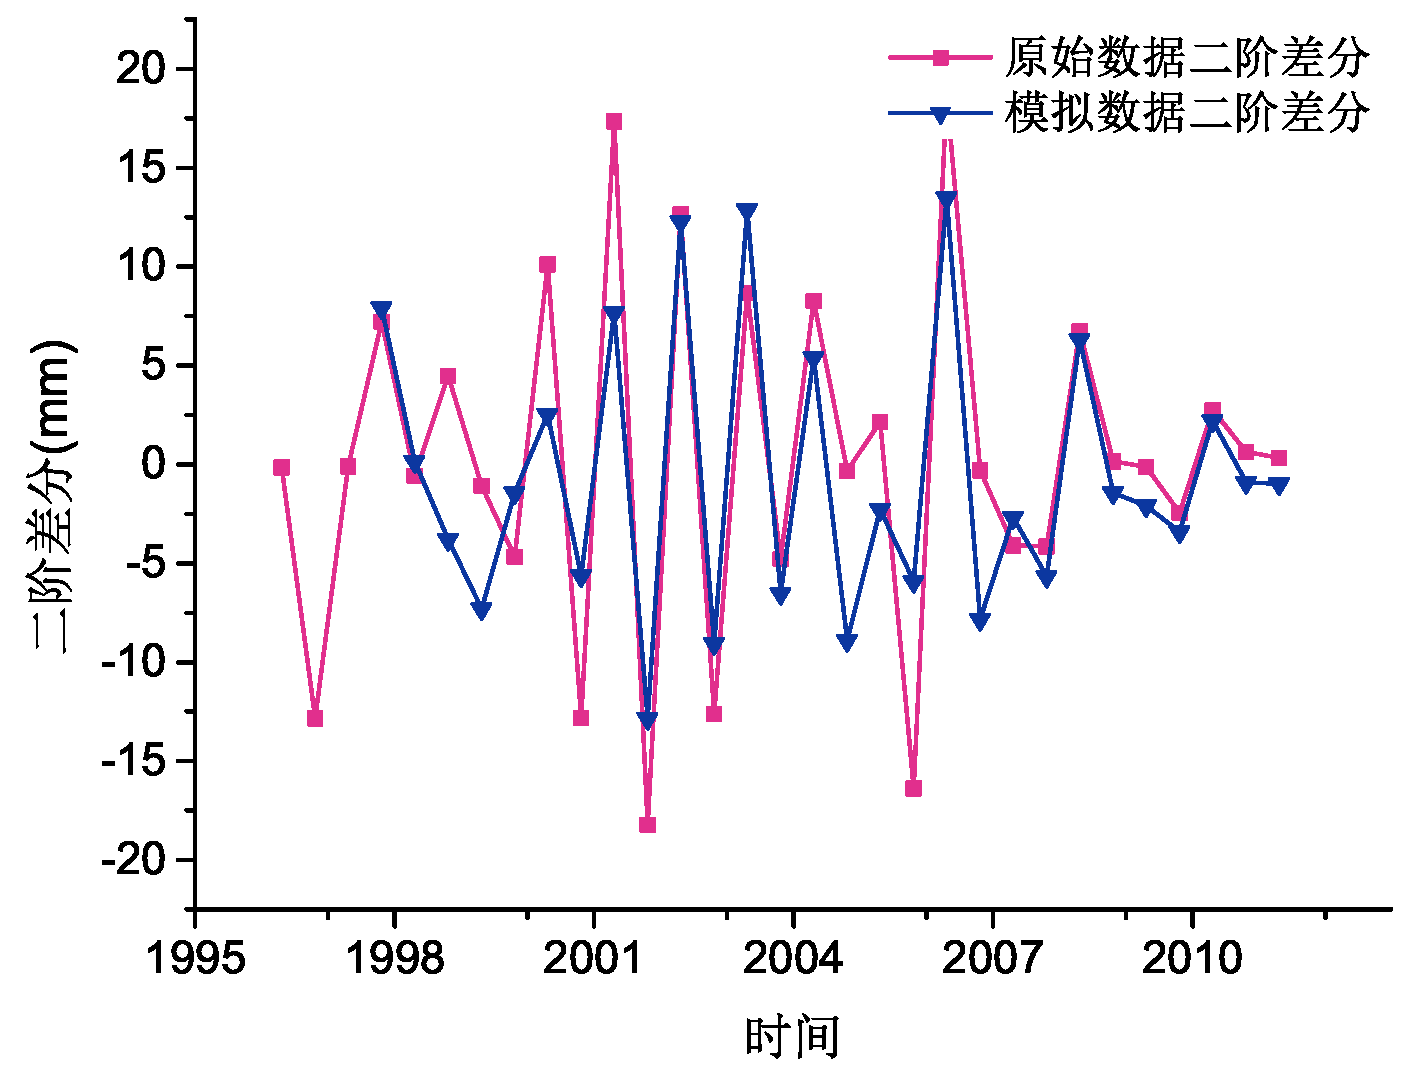
\includegraphics[width=0.7\textwidth]{chap3/diff2data.eps} \\ 
        (a)~二阶差分原始数据与预测数据图 \\
        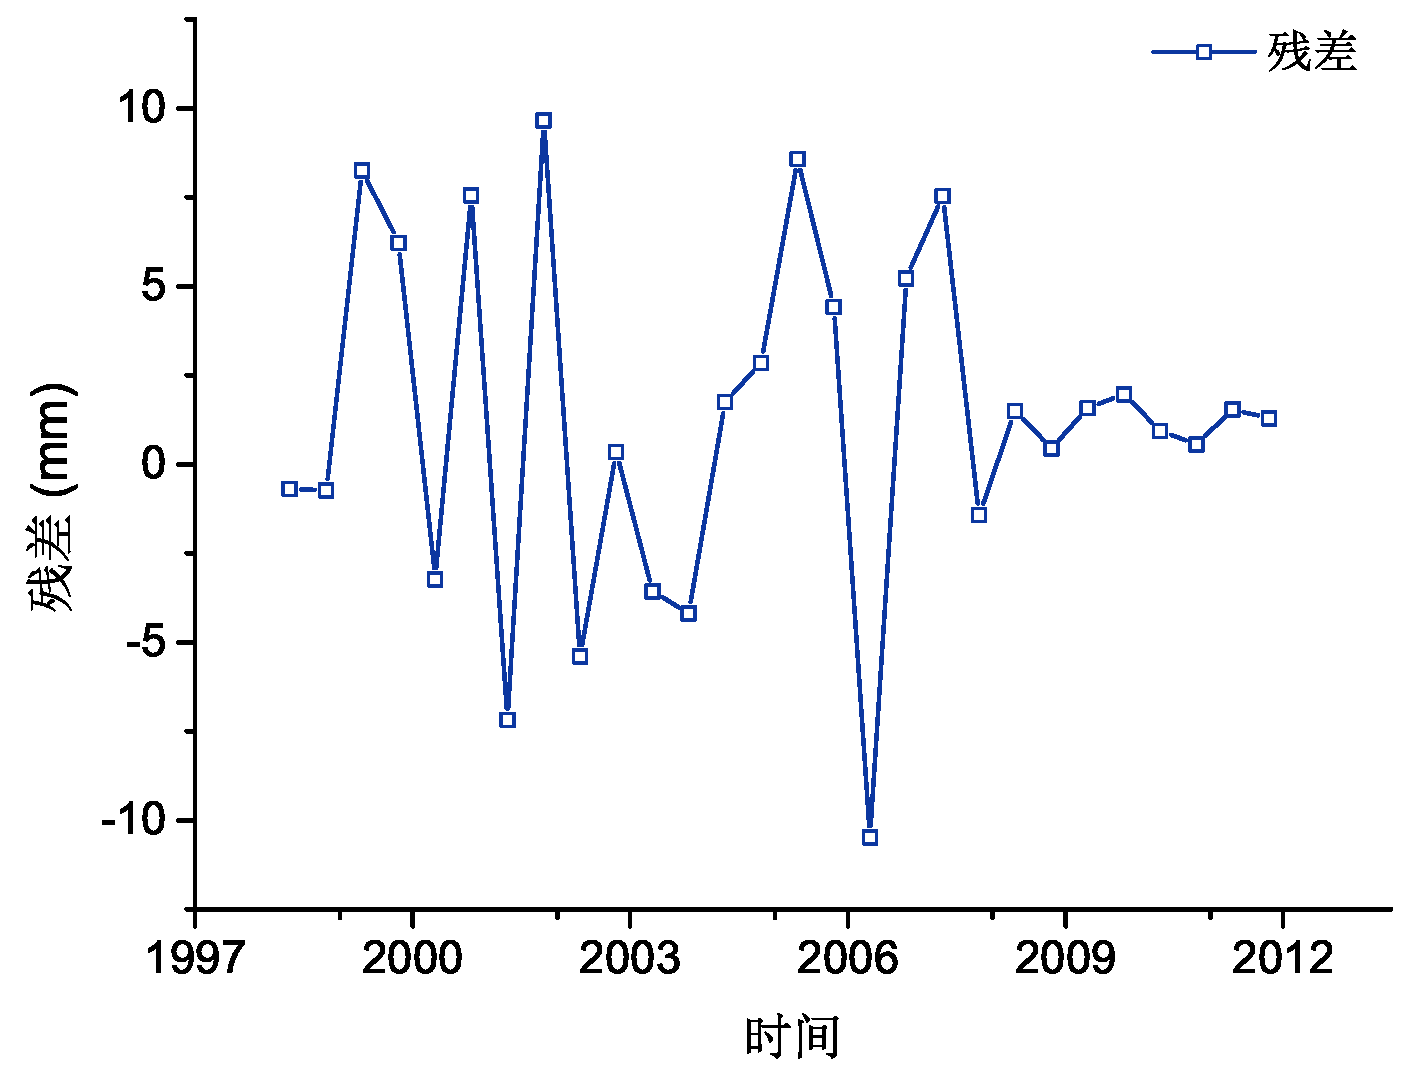
\includegraphics[width=0.7\textwidth]{chap3/ar3-residual.eps} \\ 
        (b)~二阶差分预测残差图 \\
    \end{tabular}
    \caption{AR(3)模型结果图} 
    \label{fig:AR3模型结果图} 
\end{figure}

绘制AR(3)模型计算得沉降二阶差分与原始数据二阶差分的对比图(图~\ref{fig:AR3模型结果图}a~)和二阶差分的残差图(图~\ref{fig:AR3模型结果图}b~),首先对残差进行白噪声检验,残差的自相关函数与偏相关函数,和$Q$统计量与其对应的相伴概率如表~\ref{tab:残差的自相关与偏相关系数}~所示,由表中可知,相伴概率均大于0.5\%,即在0.5\%显著性水平下,${Q}\le \chi ^{2}$,残差为白噪声。另一方面,观察自相关与偏相关函数,均落在两倍标准差范围以内,无明显规律,同样表明残差为白噪声。

综上,选择AR(3)模型模拟沉降数据是合理的,由表~\ref{tab:不同ARMA模型的参数估计}~可得时间序列模型的计算公式为
\begin{equation}
	\label{equ:ar3}
	{{\nabla }^{2}}{{Y}_{t}}=-0.89{{\nabla }^{2}}{{Y}_{t-1}}-0.60{{\nabla }^{2}}{{Y}_{t-2}}-0.51{{\nabla }^{2}}{{Y}_{t-3}}+{{\varepsilon }_{t}}
\end{equation}

可计算得沉降二阶差分模拟对应的$R^2$为0.685,还原成原始沉降数据的$R^2$为0.968。

\begin{table}[htb!]
  \centering
  \caption{残差的自相关与偏相关系数}
    \begin{tabular}{?c"m{8em}<{\centering}"m{8em}<{\centering}"c"c"c"c?}
    \thickhline
    阶数    & 自相关系数 & 偏相关系数 & AC    & PAC   & Q-Stat & Prob \bigstrut\\
    \thinhline
    1     & \multirow{12}[24]{*}{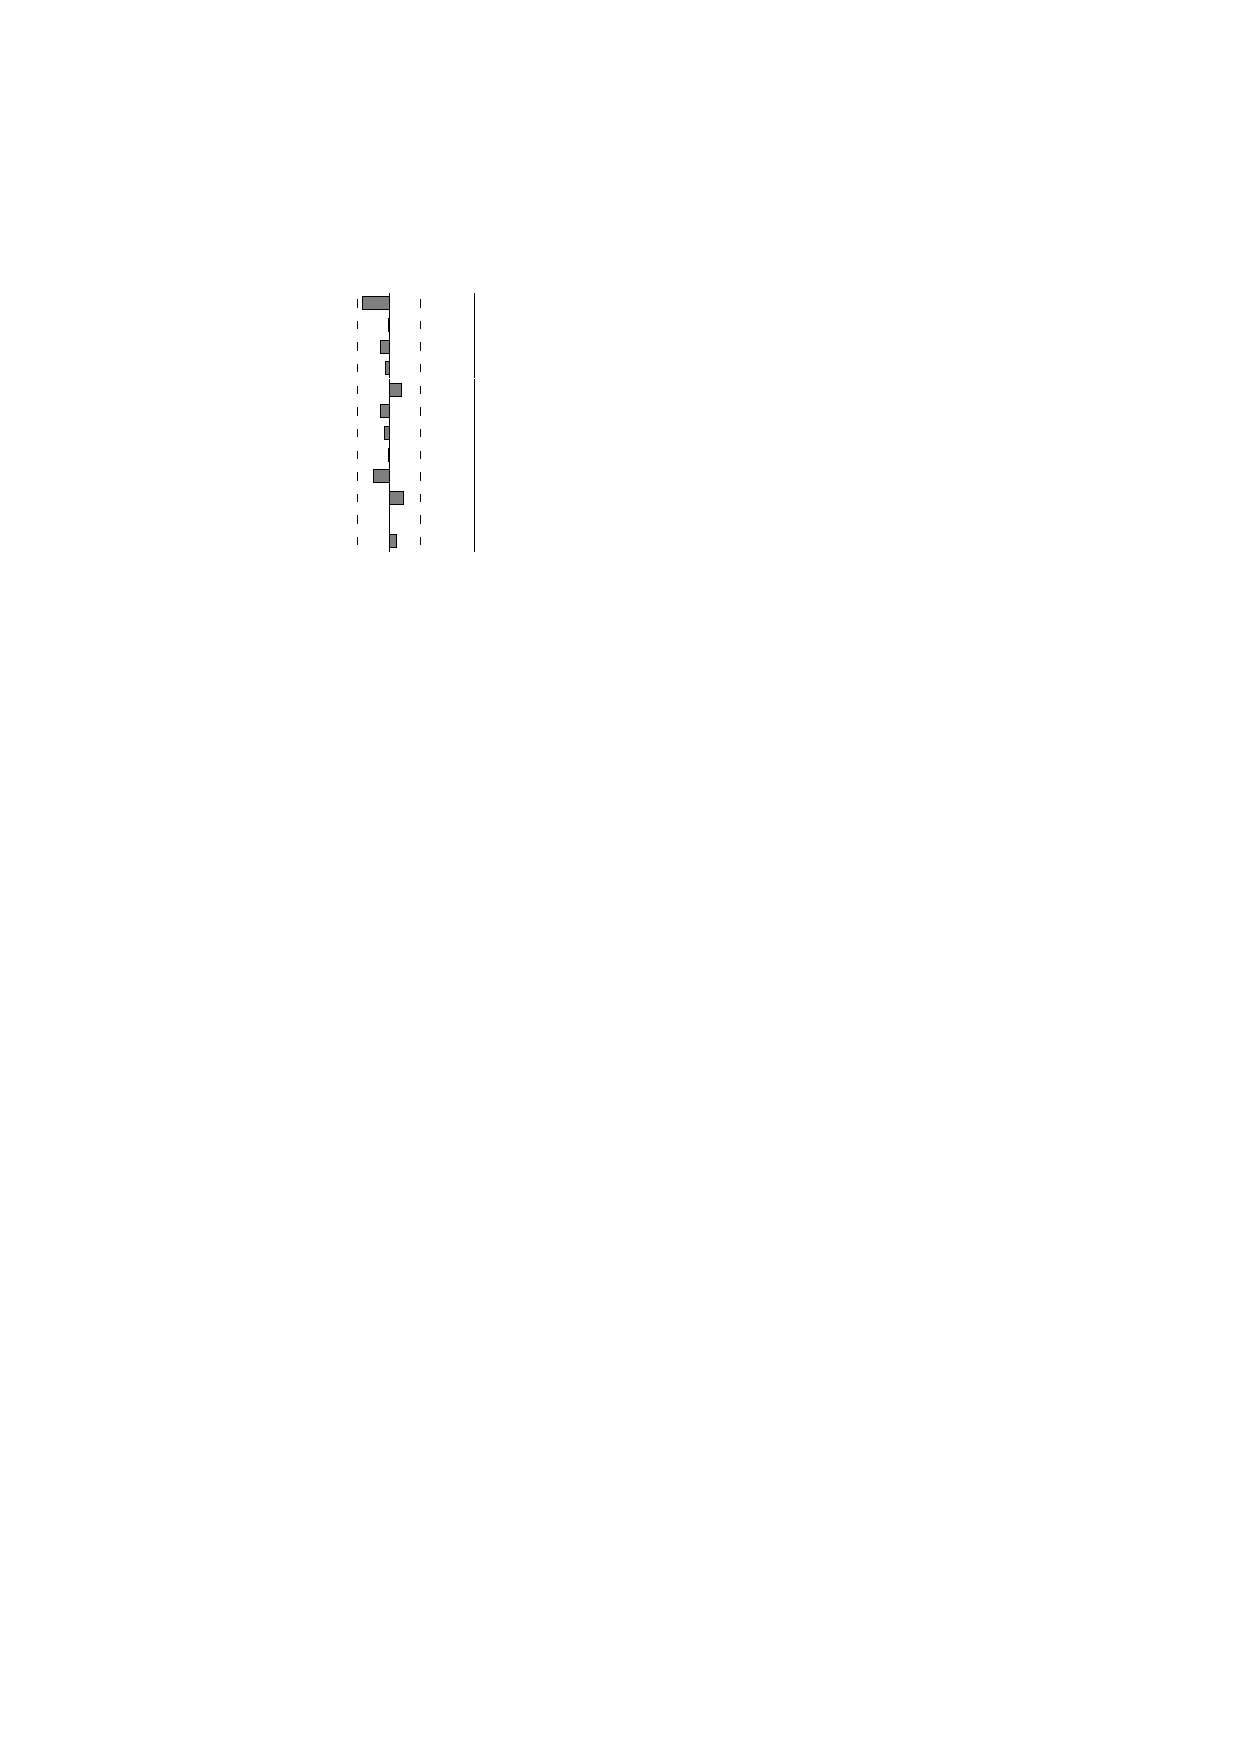
\includegraphics[width=8em,height=22.2em]{chap3/ACF3.pdf}} & \multirow{12}[24]{*}{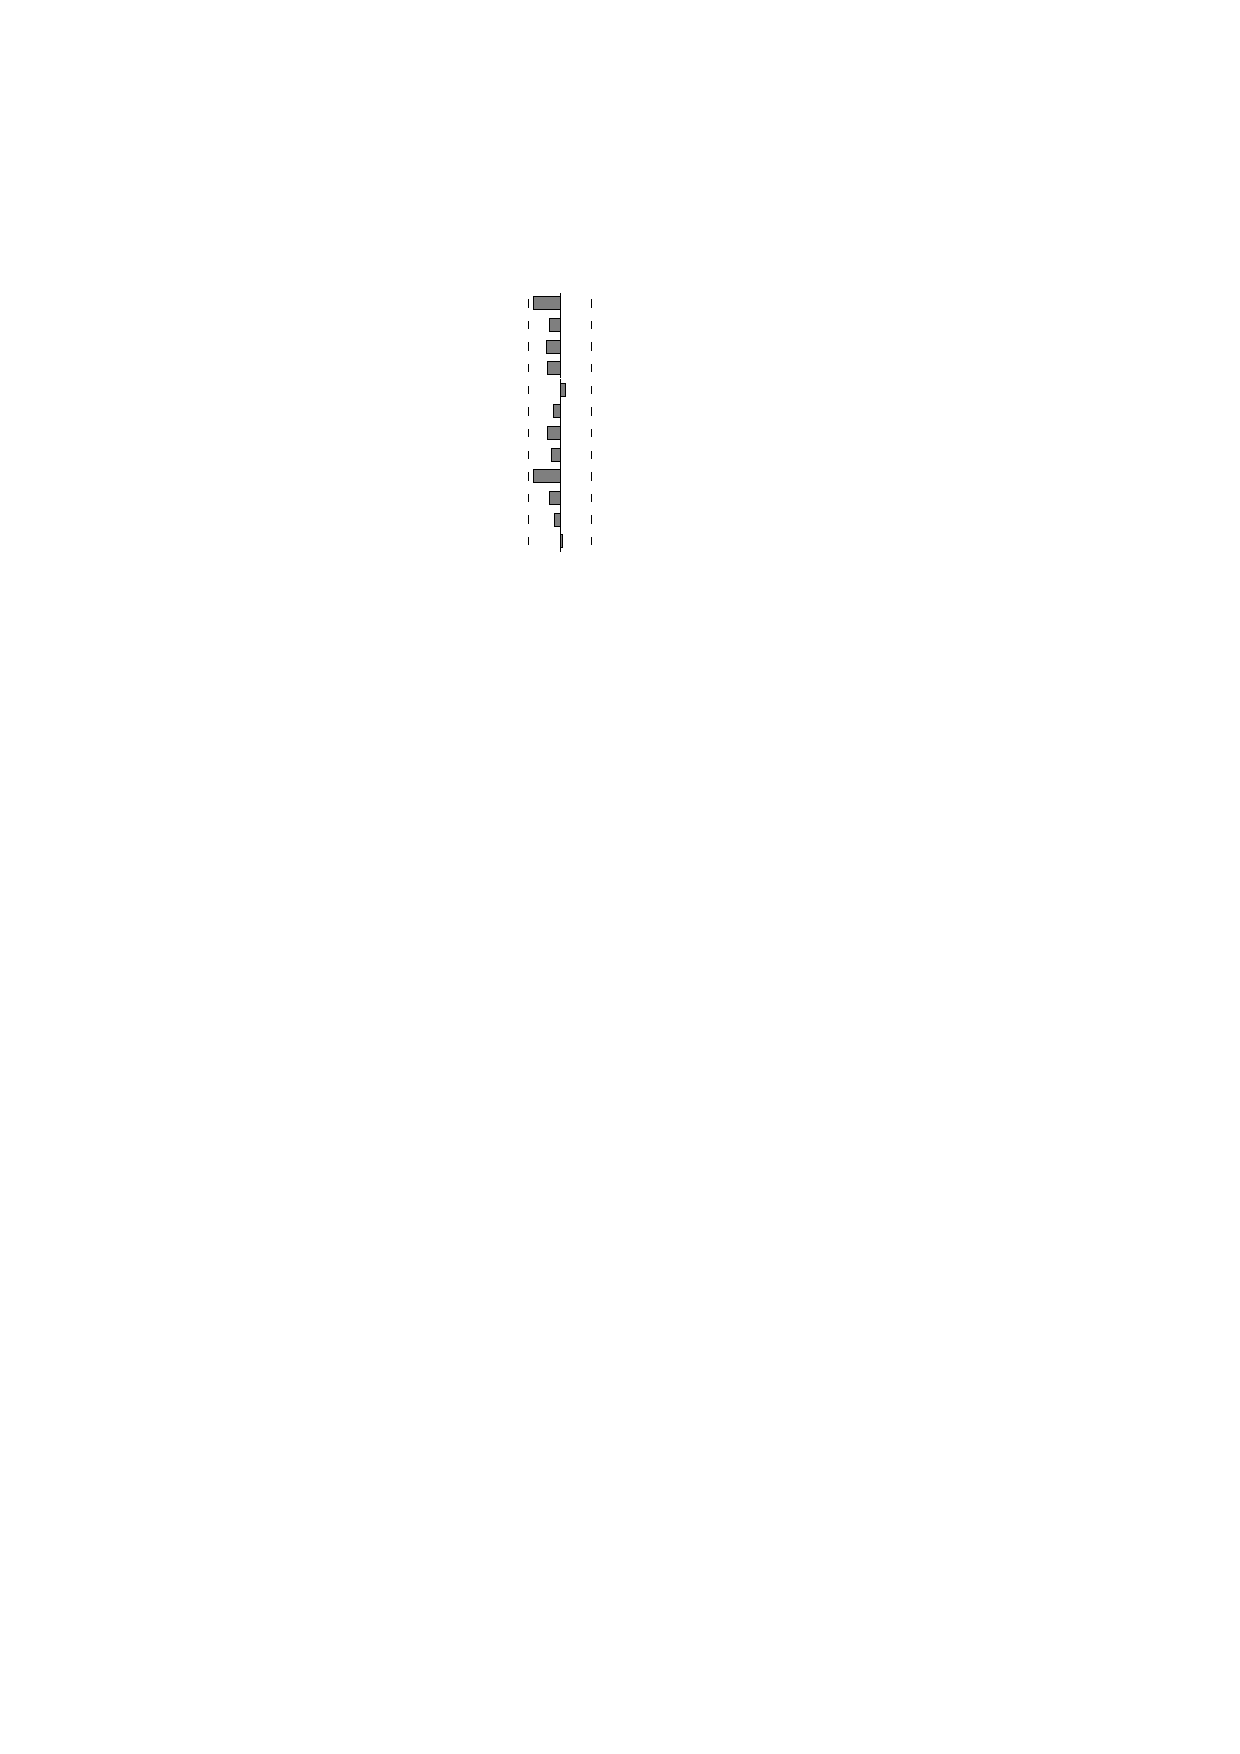
\includegraphics[width=8em,height=22.2em]{chap3/PACF3.pdf}} & -0.328 & -0.328 & 3.3387 & 0.068 \bigstrut\\
\cline{1-1}\cline{4-7}    2     &       &       & -0.008 & -0.129 & 3.3408 & 0.188 \bigstrut\\
\cline{1-1}\cline{4-7}    3     &       &       & -0.099 & -0.164 & 3.6696 & 0.299 \bigstrut\\
\cline{1-1}\cline{4-7}    4     &       &       & -0.041 & -0.158 & 3.7289 & 0.444 \bigstrut\\
\cline{1-1}\cline{4-7}    5     &       &       & 0.146 & 0.064 & 4.5043 & 0.479 \bigstrut\\
\cline{1-1}\cline{4-7}    6     &       &       & -0.114 & -0.078 & 5.0042 & 0.543 \bigstrut\\
\cline{1-1}\cline{4-7}    7     &       &       & -0.065 & -0.156 & 5.1723 & 0.639 \bigstrut\\
\cline{1-1}\cline{4-7}    8     &       &       & -0.013 & -0.109 & 5.1796 & 0.738 \bigstrut\\
\cline{1-1}\cline{4-7}    9     &       &       & -0.18 & -0.32 & 6.6194 & 0.677 \bigstrut\\
\cline{1-1}\cline{4-7}    10    &       &       & 0.167 & -0.133 & 7.9261 & 0.636 \bigstrut\\
\cline{1-1}\cline{4-7}    11    &       &       & 0.005 & -0.07 & 7.9273 & 0.72 \bigstrut\\
\cline{1-1}\cline{4-7}    12    &       &       & 0.092 & 0.022 & 8.3684 & 0.756 \bigstrut\\
    \thickhline
    \end{tabular}%
  \label{tab:残差的自相关与偏相关系数}%
\end{table}%

\subsubsection{模型预测}

采用AR(3)模型对其他沉降监测点进行预测,结果如图~\ref{fig:不同沉降监测点AR3模型拟合与预测结果}~所示,采用静态预测方法对历史数据进行拟合,采用动态预测方法预测未来数据。静态预测指的是每一次都采用真实监测数据对下一次数据进行预测,而动态预测指的下一次预测采用前面预测的结果进行迭代计算得到。由于时间序列是一种随机过程,存在不确定性,所以预测曲线给出了预测的误差范围,如图中浅蓝色区域所示,静态预测由于每一次基于真实数据,故下一次预测的误差均较小,而动态预测由于是基于预测数据,故随着预测时间越长,误差会逐渐累积,逐渐增大。图~\ref{fig:不同沉降监测点AR3模型拟合与预测结果}~展示了地铁1号线里程为 12670.10、12916.05、13145.20的三个沉降监测点的预测图,从图中可知AR(3)模型的预测效果较好,对于沉降二次差分的拟合$R^2$在0.6以上,对原始沉降数据的拟合$R^2$在0.95以上。

\begin{figure}[htbp] 
    \centering 
    \begin{tabular}{c} 
        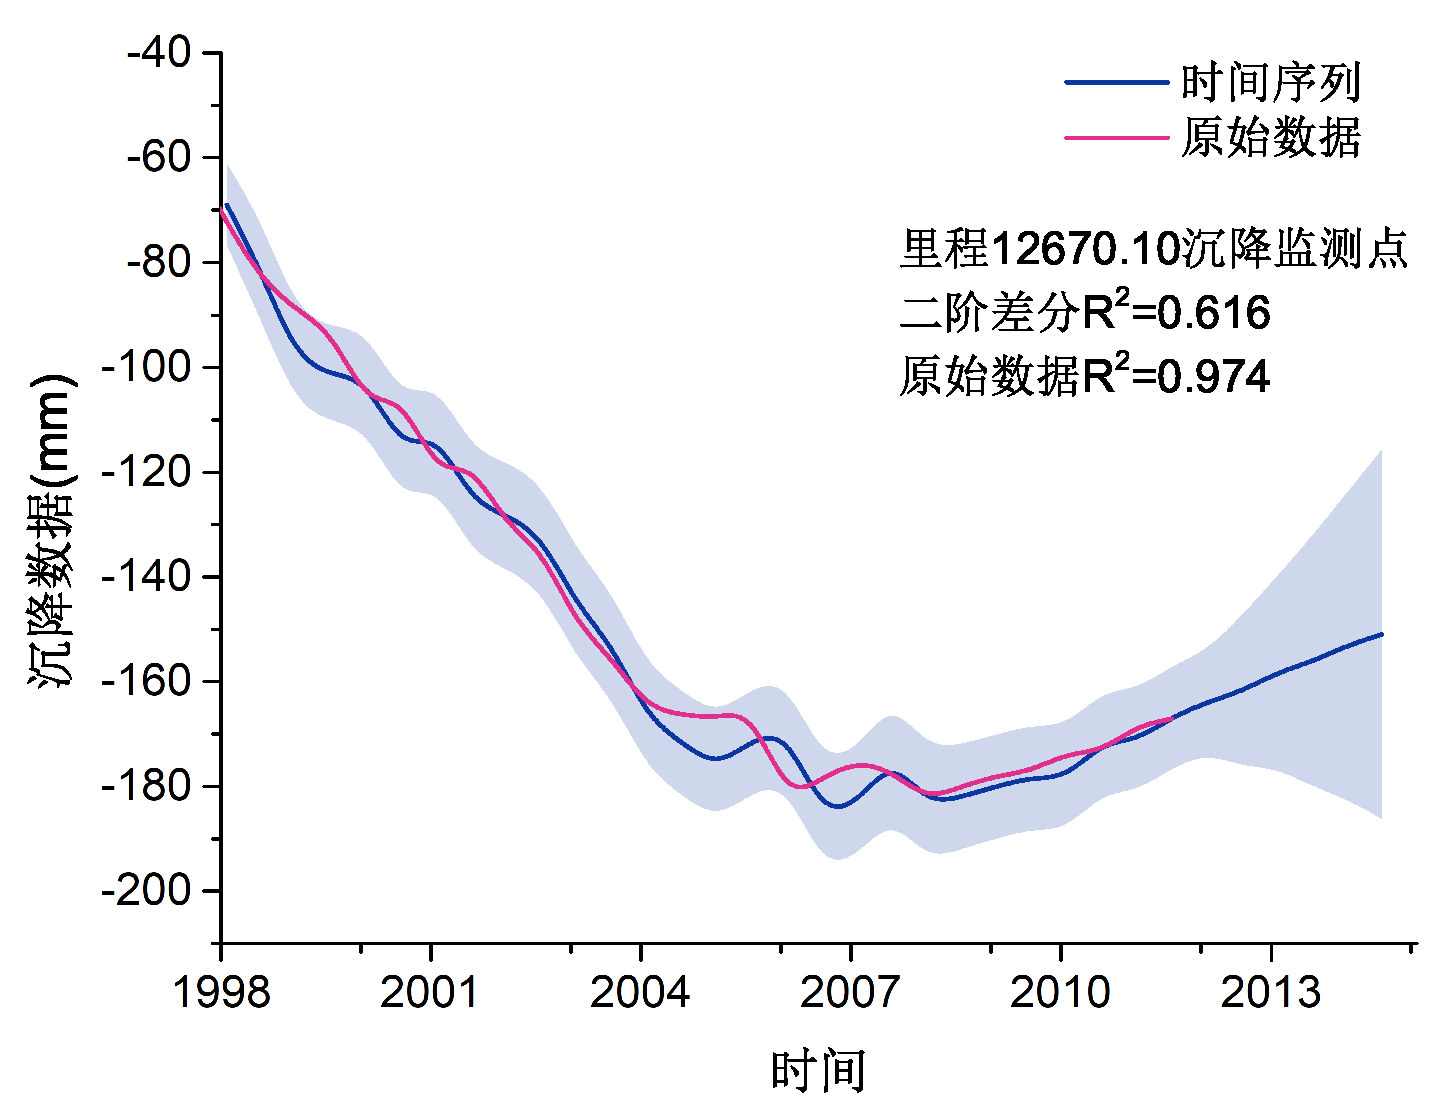
\includegraphics[width=0.61\textwidth]{chap3/sett-12670.10.eps} \\ 
        (a)~里程12670.10沉降监测点数据 \\
        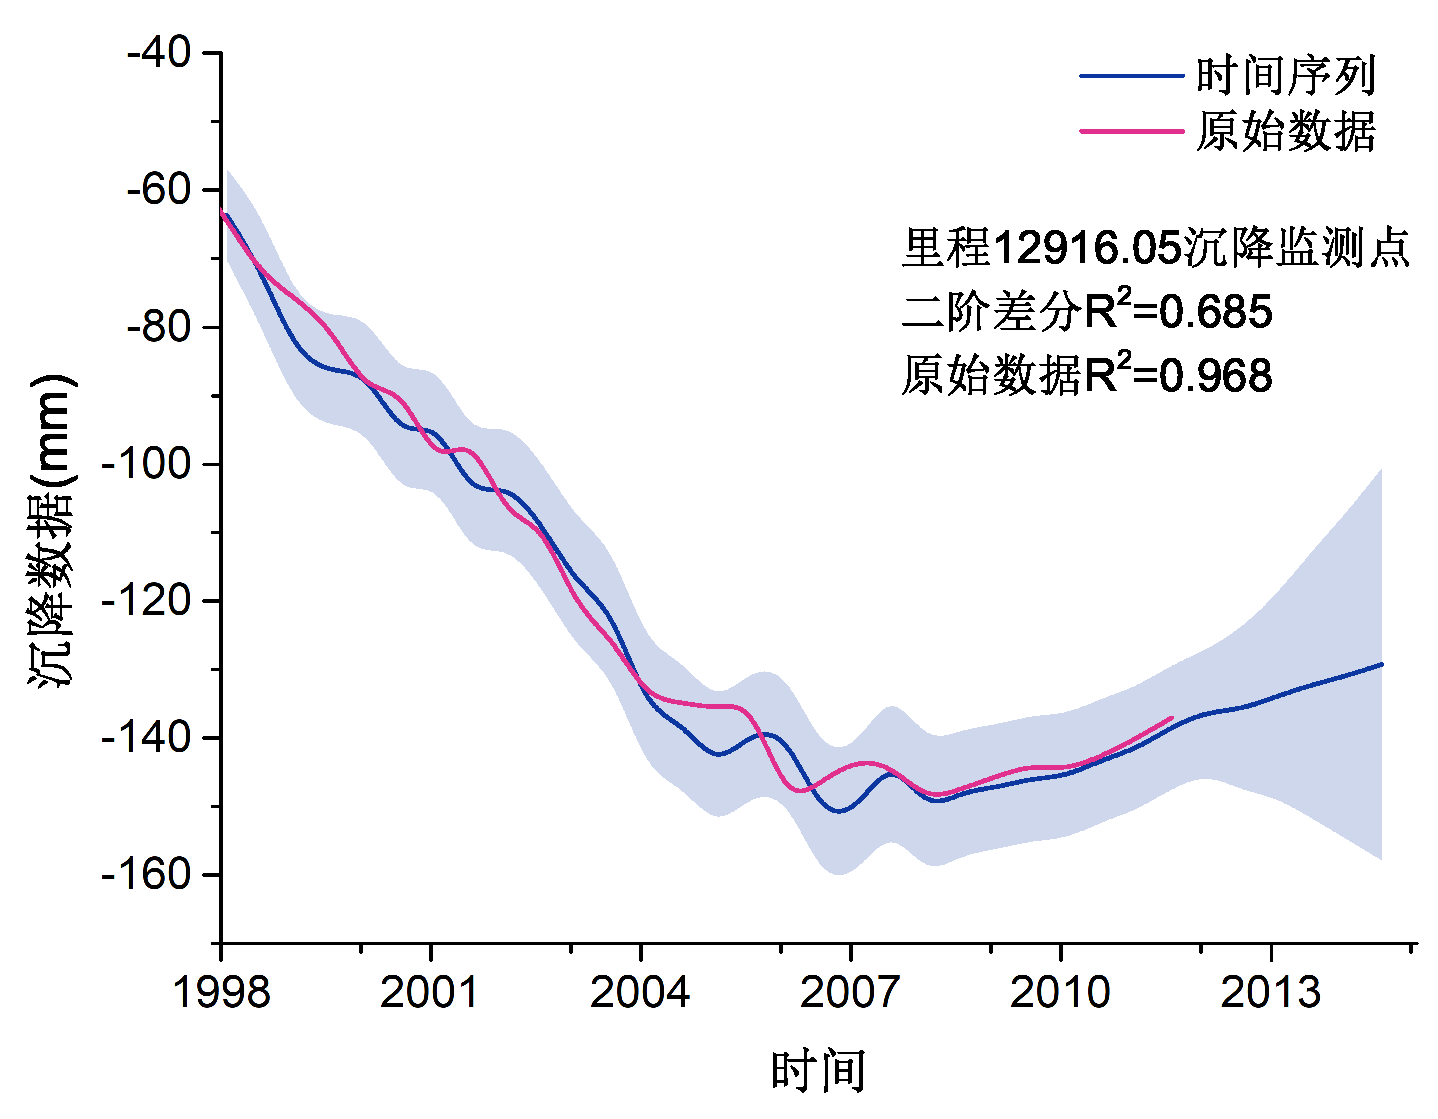
\includegraphics[width=0.61\textwidth]{chap3/sett-12916.05.eps} \\ 
        (b)~里程12916.05沉降监测点数据 \\
        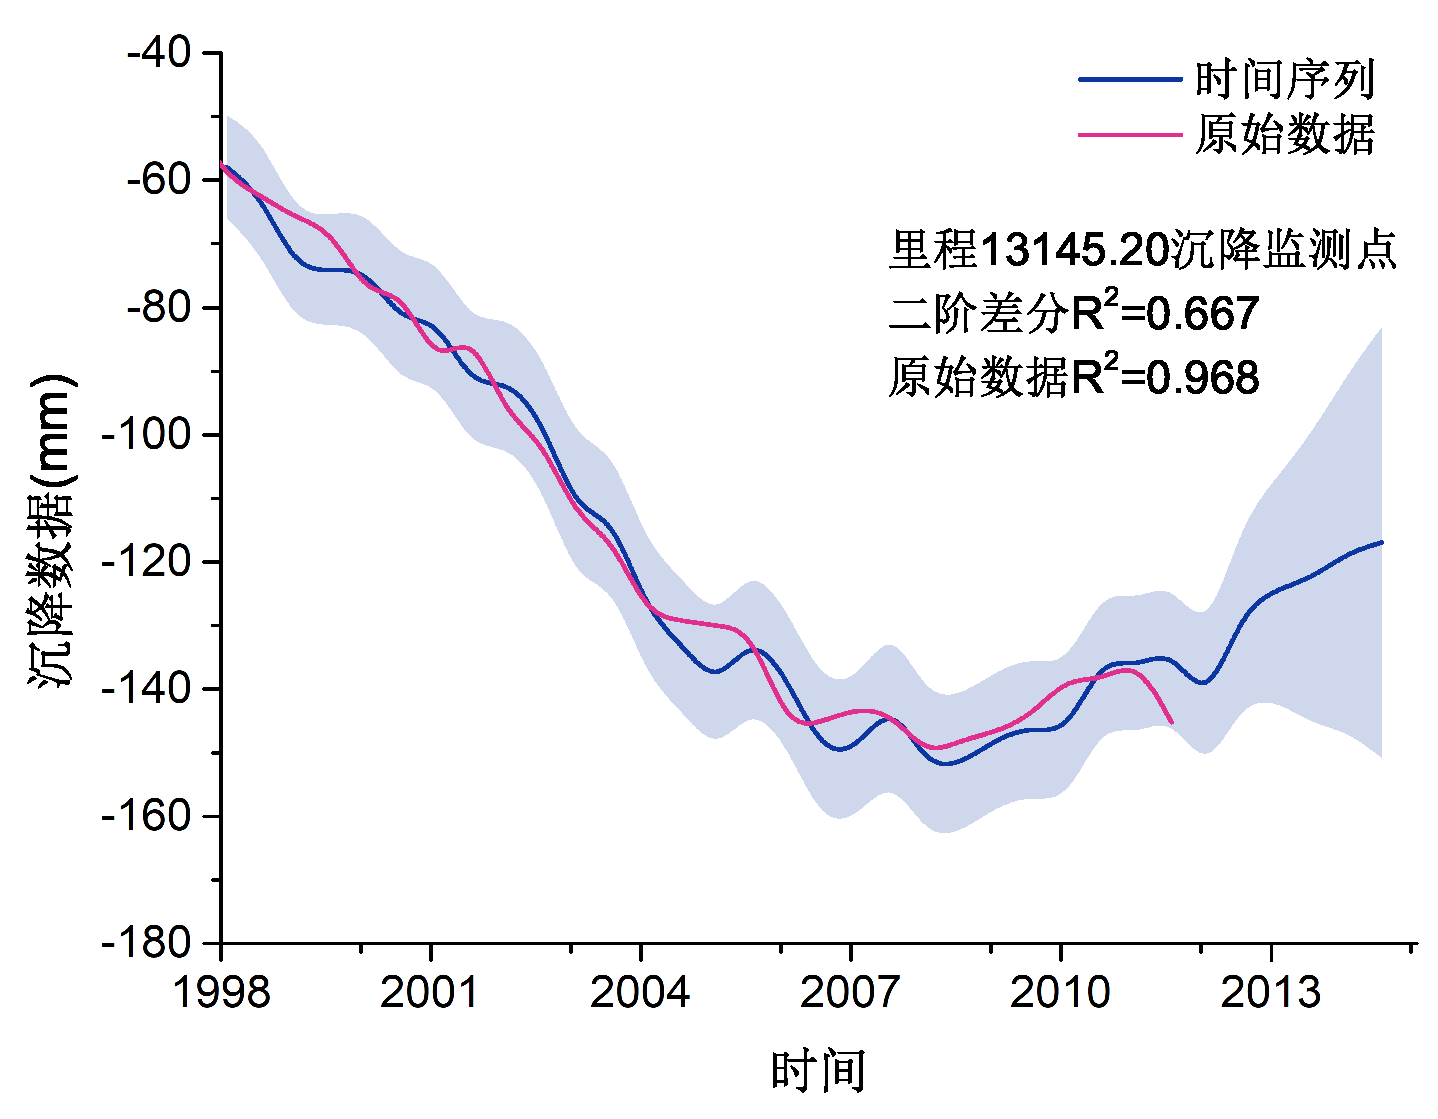
\includegraphics[width=0.61\textwidth]{chap3/sett-13145.20.eps} \\ 
        (c)~里程13145.20沉降监测点数据 \\
    \end{tabular}
    \caption{不同沉降监测点AR(3)模型拟合与预测结果} 
    \label{fig:不同沉降监测点AR3模型拟合与预测结果} 
\end{figure}

%%%%%%%%%%%%%%%%%%%%%%%%%%%%%%%%%%%%%%%%%%%%%%%%%%%%%%%%%%%%%%%%%%%
\section{考虑空间效应的结构-向量时间序列模型}

%+++++++++++++++++++++++++++++++++++++++++++++++++++++++++++++++++%
\subsection{基本原理}

\subsubsection{向量时间序列}
\label{chap:var}

向量时间序列是根据数据统计性建立的模型,向量时间序列将研究系统的每一个对象作为系统内所有对象的滞后值函数,将单个变量的时间序列推广到多个时间序列组成的向量时间序列。Sims(\citeyear{sims1980macroeconomics})首先提出向量时间序列的概念,并将其运用于经济领域的动态分析应用中,该模型可用于预测互相联系的序列,并且分析不同系统变量扰动对系统的动态冲击,在经济领域得到较好应用。

首先介绍向量时间序列中的向量自回归(VAR)模型,$p$阶VAR模型VAR(p)的数学表达式为
\begin{equation}
	\label{equ:varp}
	{{y}_{t}}={{\Phi }_{1}}{{y}_{t-1}}+\cdots +{{\Phi }_{p}}{{y}_{t-p}}+H{{x}_{t}}+{{\varepsilon }_{t}},t=1,2,\cdots ,T
\end{equation}
式中:$y_t$是$k$维内生变量列向量,$x_t$是$d$维外生变量列向量,$p$是滞后阶数,$T$是样本个数。$k\times k$维矩阵${\Phi }_1,{\Phi }_2,\cdots ,{\Phi }_p$和$k\times d$维矩阵$H$是待估计的系数矩阵。${\varepsilon }_{t}$是$k$维的扰动列向量,同期扰动项之间相关,但不与自己的滞后值相关,定义$\sum$为${\varepsilon }_{t}$的协方差矩阵,为$k\times k$的正定矩阵,展开式~\ref{equ:varp}~可以得到
\begin{equation}
	\left( \begin{array}{*{35}{l}}
   {{y}_{1t}}  \\
   {{y}_{2t}}  \\
   \cdots   \\
   {{y}_{kt}}  \\
\end{array} \right)={{\Phi }_{1}}\left( \begin{array}{*{35}{l}}
   {{y}_{1t-1}}  \\
   {{y}_{2t-1}}  \\
   \cdots   \\
   {{y}_{kt-1}}  \\
\end{array} \right)+\cdots +{{\Phi }_{p}}\left( \begin{array}{*{35}{l}}
   {{y}_{1t-p}}  \\
   {{y}_{2t-p}}  \\
   \cdots   \\
   {{y}_{kt-p}}  \\
\end{array} \right)+H\left( \begin{array}{*{35}{l}}
   {{x}_{1t}}  \\
   {{x}_{2t}}  \\
   \cdots   \\
   {{x}_{kt}}  \\
\end{array} \right)+\left( \begin{array}{*{35}{l}}
   {{\varepsilon }_{1t}}  \\
   {{\varepsilon }_{2t}}  \\
   \cdots   \\
   {{\varepsilon }_{kt}}  \\
\end{array} \right)
\end{equation}
从式中可知,含有$k$个时间序列的VAR(p)模型是由$k$个方程组组成的。将$y_t$对$x_t$作回归后的残差表达式为
\begin{equation}
	{{\tilde{y}}_{t}}={{\tilde{\Phi }}_{1}}{{\tilde{y}}_{t-1}}+\cdots +{{\tilde{\Phi }}_{p}}{{\tilde{y}}_{t-p}}+{{\tilde{\varepsilon }}_{t}}
\end{equation}
式中:$\tilde{y}_{t}$是$y_t$对$x_t$回归的残差,${{\tilde{\varepsilon }}_{t}}$是残差回归的扰动项,为了叙述方便,本文不考虑外生变量的影响,则重新将VAR方程写为
\begin{gather}
	\label{equ:varsimple}
	{{y}_{t}}={{\Phi }_{1}}{{y}_{t-1}}+\cdots +{{\Phi }_{p}}{{y}_{t-p}}+{{\varepsilon }_{t}} \\
	{\Phi }(L)y_t={\varepsilon }_{t}
\end{gather}
式中:${\Phi }(L)y_t=I_k-{\Phi }_{1}L-\cdots -{\Phi }_{p}L^p$是滞后算子$L$的$k\times k$参数矩阵,如果行列式$\det \left[ \Phi (L) \right]$的根都在单位圆外,则式~\ref{equ:varsimple}~满足平稳性的条件,并可以表示成无穷阶的向量滑动平均VMA($\infty $)形式
\begin{gather}
	\label{equ:vmap}
	{{y}_{t}}=A(L){{\varepsilon }_{t}} \\ 
	A(L)=\Phi {{(L)}^{-1}}={{A}_{0}}+{{A}_{1}}L+{{A}_{2}}{{L}^{2}}+\cdots 
\end{gather}

\subsubsection{结构时间序列}

在~\ref{chap:var}~小节中,可以由式~\ref{equ:varsimple}~看出,没有建立当期变量之间的关系,而将其归在扰动当中,VAR模型并未能提取所有物理意义,故将式~\ref{equ:varp}~称为简化式模型。另一方面,由于现实数据之间是存在关联性的,一般可通过合理的物理意义对估计参数空间施加约束,减少所要估计的参数数量。下面介绍VAR的结构式模型,其包含当前变量的信息。

对于$k$个变量,$p$阶的结构-向量自回归SVAR(p)为
\begin{equation}
	\label{equ:svarp}
	{{C}_{0}}{{y}_{t}}={{\Gamma }_{1}}{{y}_{t-1}}+{{\Gamma }_{2}}{{y}_{y-2}}+\cdots +{{\Gamma }_{p}}{{y}_{t-p}}+{{u}_{t}},\quad t=1,2,\cdots ,T
\end{equation}
其中,
\begin{gather}
  {{C}_{0}}=\left[ \begin{matrix}
   1 & -{{c}_{12}} & \cdots  & -{{c}_{1k}}  \\
   -{{c}_{21}} & 1 & \cdots  & -{{c}_{2k}}  \\
   \vdots  & \vdots  & \ddots  & \vdots   \\
   -{{c}_{k1}} & -{{c}_{k2}} & \cdots  & 1  \\
\end{matrix} \right],\quad {{\Gamma }_{i}}=\left[ \begin{matrix}
   \gamma _{11}^{(i)} & \gamma _{12}^{(i)} & \cdots  & \gamma _{1k}^{(i)}  \\
   \gamma _{21}^{(i)} & \gamma _{22}^{(i)} & \cdots  & \gamma _{2k}^{(i)}  \\
   \vdots  & \vdots  & \ddots  & \vdots   \\
   \gamma _{k1}^{(i)} & \gamma _{k2}^{(i)} & \cdots  & \gamma _{kk}^{(i)}  \\
\end{matrix} \right], \nonumber \\ 
 i=1,2,\cdots ,p,\quad {{u}_{t}}=\left[ \begin{matrix}
   {{u}_{1t}}  \\
   {{u}_{2t}}  \\
   \vdots   \\
   {{u}_{kt}}  \\
\end{matrix} \right] \nonumber
\end{gather}
式中:$y_t$均是平稳时间序列;$u_t$是白噪声序列,假设其方差-协方差矩阵为单位矩阵$I_k$,${u}_{1t},{u}_{2t},\cdots {u}_{kt}$之间不相关;$c_{jk}$系数表示第$j$个变量的单位变化对第$k$个变量的作用;$\gamma _{jk}^{(i)}$表示第$j$个变量的单位变化对第$k$个变量的$i$阶滞后作用。可以将式~\ref{equ:svarp}~写成滞后算子形式
\begin{equation}
	C(L){{y}_{t}}={{u}_{t}},\quad E({{u}_{t}}{{{u}'}_{t}})={{I}_{k}}
\end{equation}
式中:$C(L)={{C}_{0}}-{{\Gamma }_{1}}L-{{\Gamma }_{2}}{{L}^{2}}-\cdots -{{\Gamma }_{p}}{{L}^{p}}$,$C(L)$是滞后算子$L$的$k\times k$的参数矩阵。$C_0$是主对角线元素为1的矩阵。如果矩阵多项式$C(L)$可逆,可写出SVAR的无穷阶的结构-向量滑动平均SVMA($\infty $)模型
\begin{equation}
	\label{equ:svmap}
	{{y}_{t}}=B(L){{u}_{t}}
\end{equation}
式中:
\begin{equation}
	B(L)=C{{(L)}^{-1}},\quad B(L)={{B}_{0}}+{{B}_{1}}L+{{B}_{2}}{{L}^{2}}+\cdots ,\quad {{B}_{0}}=C_{0}^{-1}
\end{equation}
联立式~\ref{equ:vmap}~和式~\ref{equ:svmap}~可得最终典型的SVAR模型
\begin{equation}
	\label{equ:finalsvar}
	A(L){\varepsilon }_{t}=B(L){u}_{t}
\end{equation}
由于$A_0=I_k$,可知
\begin{equation}
	\label{equ:ABrela}
	{A}_{0}{\varepsilon }_{t}={\varepsilon }_{t}={B_0}{u_t},\quad {B}_0^{-1}{\varepsilon }_{t}=u_t
\end{equation}

更一般的情况,假设有两个$k\times k$的矩阵$A$和$B$,将$A$乘以公式~\ref{equ:varsimple}~得到
\begin{equation}
	A{\Phi }(L)y_t=A{\varepsilon }_{t}
\end{equation}
如果矩阵$A$、$B$满足$A{\varepsilon }_{t}=Bu_t,E(u_t)=0,E(u_tu'_t)=I_k$,则将模型称为AB-型的SVAR模型。

%+++++++++++++++++++++++++++++++++++++++++++++++++++++++++++++++++%
\subsubsection{模型识别}

对于$k$元$p$阶的VAR模型(式~\ref{equ:varsimple}),利用极大似然方法,需要的估计参数个数为$k^2p+(k+k^2)/2$,对于相应的$k$元$p$阶的SVAR模型(式~\ref{equ:svarp})所需的参数个数为$k^2p+k^2$,结合式~\ref{equ:finalsvar}~,根据秩条件,要得到SVAR模型参数的唯一估计,需满足简化式的未知参数不比结构式的未知参数多。因此需对SVAR模型进行约束,至少的约束个数为$k^2p+(k+k^2)/2$-$k^2p+k^2$=$k(k-1)/2$。这些约束可以是施加给当期变量(短期约束),也可以是给时滞变量(长期约束)。特别的,对于AB型SVAR,需要增加$2k^2-k(k+1)/2$个约束。

联立式~\ref{equ:finalsvar}~和式~\ref{equ:ABrela}~可得
\begin{equation}
	A(L)B_0u_t=B(L)u_t
\end{equation}
式中:$A(L)$和$B(L)$分别是VMA($\infty $)和SVMA($\infty $)的滞后多项式,由该公式可以推断出
\begin{equation}
	\label{equ:ABrela2}
	A_iB_0=B_i, \quad i=0,1,2,\cdots
\end{equation}
如果$B_0$已知,可以通过式~\ref{equ:ABrela}~和式~\ref{equ:ABrela2}~计算得到滞后多项式和结构模型的新息$u_t$。故只需对$B_0$进行约束即可识别整个系统。

短期约束可以直接施加在矩阵$B_0$,表示变量对结构模型的同期响应,常见的约束方式是0约束排除方法;由于$B_0=C_0^{-1}$,也可以通过对$C_0$施加约束条件实现短期约束。对于长期约束,一般是通过施加在系数矩阵$B_i(i=1,2,\cdots )$上。

%+++++++++++++++++++++++++++++++++++++++++++++++++++++++++++++++++%
\subsubsection{脉冲响应分析}

VAR模型和SVAR模型可以分析某一变量的冲击对系统的影响,主要的思想是分析扰动项的变化对各变量的影响。下面以两个时间序列变量$x_t$、$z_t$的模型说明脉冲响应分析的方法。
\begin{align}
  \label{equ:varexample}
  & {{x}_{t}}={{a}_{1}}{{x}_{t-1}}+{{a}_{2}}{{x}_{t-2}}+{{b}_{1}}{{z}_{t-1}}+{{b}_{2}}{{z}_{t-2}}+{{\varepsilon }_{1t}} \\ 
 & {{z}_{t}}={{c}_{1}}{{x}_{t-1}}+{{c}_{2}}{{x}_{t-2}}+{{d}_{1}}{{z}_{t-1}}+{{d}_{2}}{{z}_{t-2}}+{{\varepsilon }_{2t}} \nonumber
\end{align}
式中:$a_i$,$b_i$,$c_i$,$d_i$是待评估参数,${\varepsilon }_{1t}$和${\varepsilon }_{2t}$是扰动项。假设该模型从0时间点开始,$x_{-1}=x_{-2}=z_{-1}=z_{-2}=0$,在0时间点又扰动项${\varepsilon }_{10}=1,{\varepsilon }_{20}=0$,之后扰动项均为0,${\varepsilon }_{1t}={\varepsilon }_{2t}=0(t=1,2,\cdots )$,上述则在0时间给$x$施加脉冲,在$t=0$时:
\begin{equation}
	x_0=1,\quad z_0=0 \nonumber
\end{equation}

将上式代入式~\ref{equ:varexample}~,得当$t=1$时:
\begin{equation}
	x_1=a_1,\quad z_1=c_1 \nonumber
\end{equation}

再把上式结果代入式~\ref{equ:varexample}~,得当$t=2$时:
\begin{equation}
	x_2=a_1^2+a_2+b_1c_1,\quad z_2=c_1a_1+c_2+d_1c_1 \nonumber
\end{equation}

循环执行上述过程,可分别求得$x_0,x_1,x_2,x_3,\cdots $和$z_0,z_1,z_2,z_3,\cdots $,称之为由$x$的脉冲引起的$x$和$z$的响应函数。同样的,可采用类似方法求得不同时期,不同变量脉冲引起的响应函数。

%+++++++++++++++++++++++++++++++++++++++++++++++++++++++++++++++++%
\subsection{盾构隧道结构-向量时间序列模型建模}

\subsubsection{VAR模型}

VAR/SVAR模型的建立过程跟ARMA模型类似,可以分为VAR模型建立、AR根平稳性检验(Liitkepohl,\citeyear{liitkepohl1991introduction})、滞后阶数确定、SVAR模型参数估计、脉冲分析等,如图~\ref{fig:VARSVAR模型建模流程图}~所示。

\begin{figure}[htb!]
    \centering
    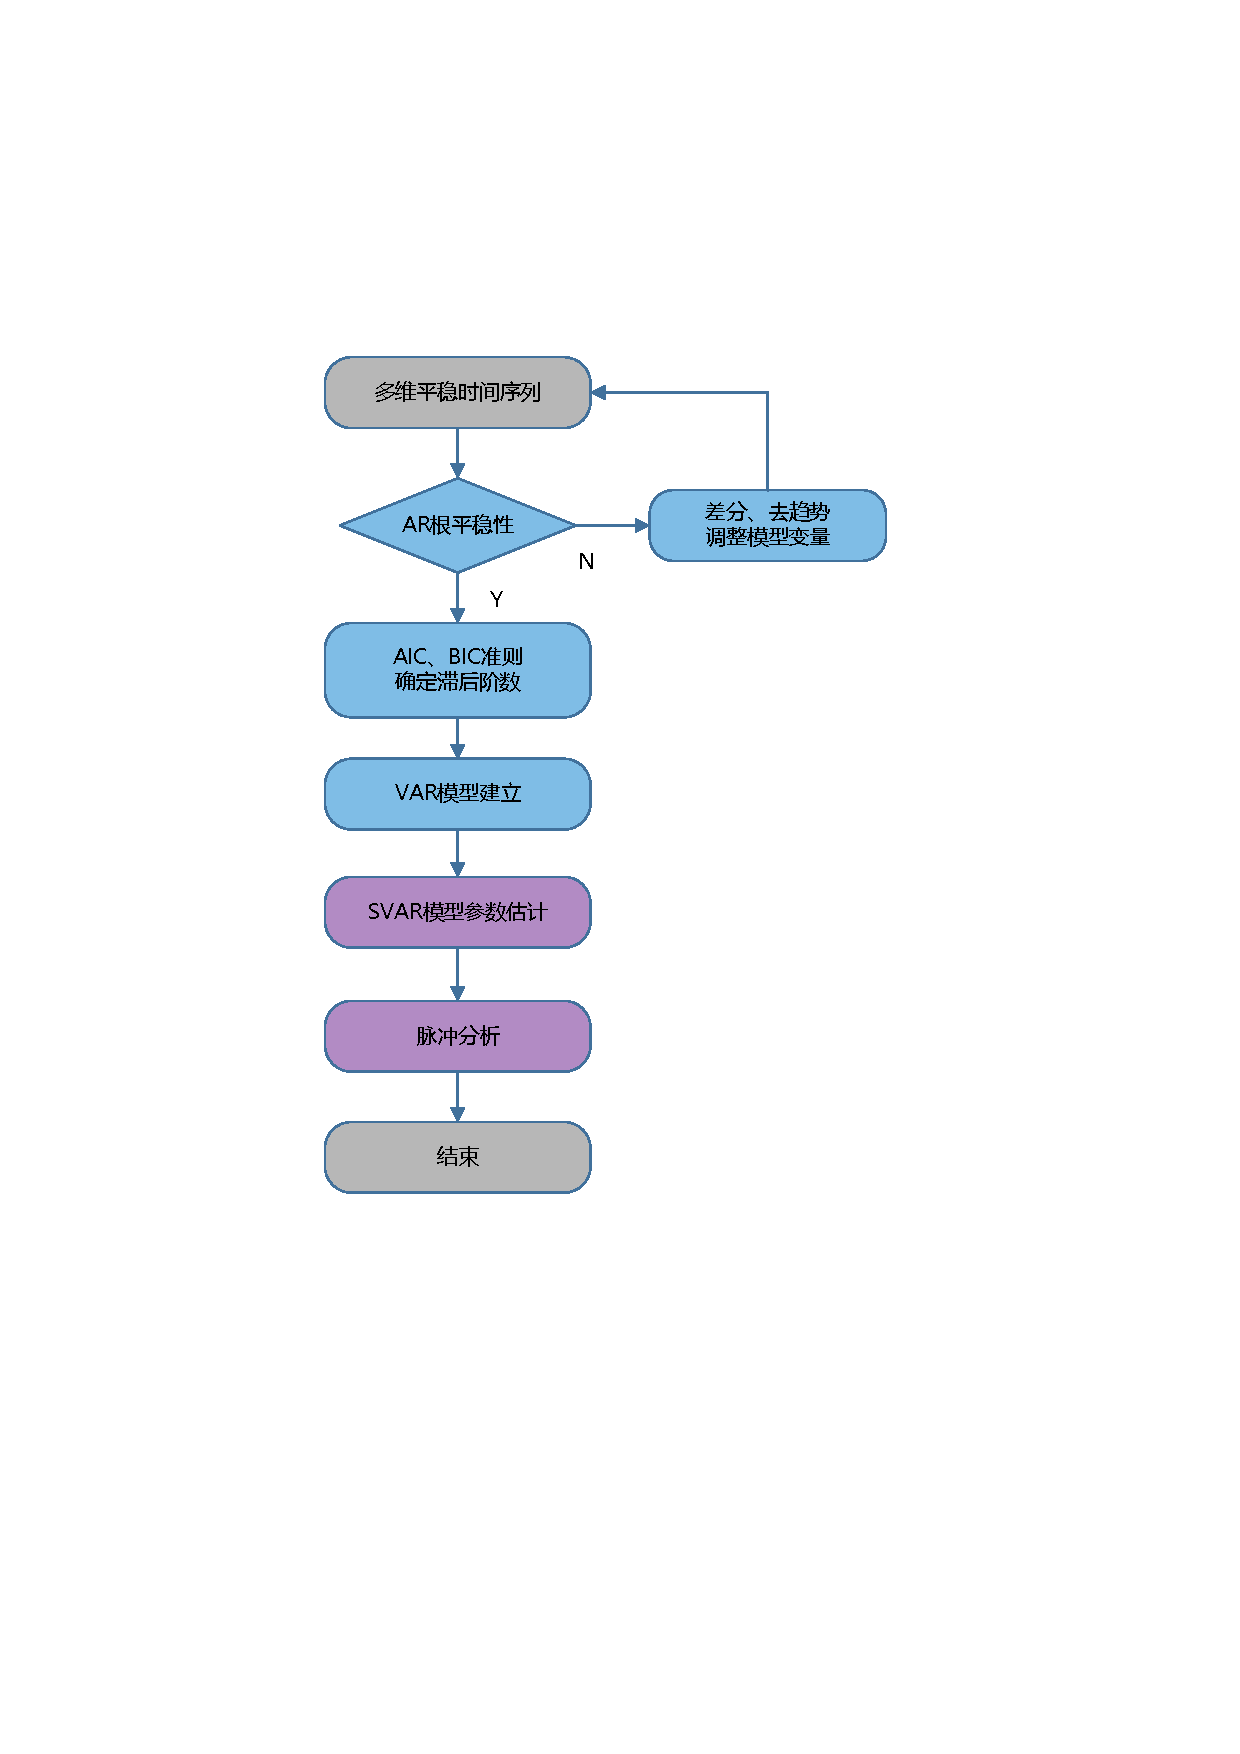
\includegraphics[width=0.6\textwidth]{chap3/var-process.pdf}
    \caption{VAR/SVAR模型建模流程图}
    \label{fig:VARSVAR模型建模流程图}
\end{figure}

由~\ref{chap:armatunnel}~小节可知,沉降数据的二阶差分为平稳序列,考虑到目前上海1号线一个监测点只有33次的监测数据,为了更好估计模型参数,本节只选择三个相邻的监测点时间序列作为研究,依次为里程12916.05、12920.75、12944.4的三个沉降监测点,分别记为$s_1$、$s_2$和$s_3$。对于滞后阶数,如果滞后阶数选择过大,则待估计参数会较多,给参数估计带来困难;如果滞后阶数选择过小,则不能保证模型的准确性,表~\ref{tab:VAR模型最优滞后阶数确定}~所示为根据不同准则计算的滞后阶数值,综合考虑选择滞后阶数为3。因此,盾构隧道沉降的VAR模型为
\begin{equation}
	\left( \begin{matrix}
   {{\nabla }^{2}}{{s}_{1t}}  \\
   {{\nabla }^{2}}{{s}_{2t}}  \\
   {{\nabla }^{2}}{{s}_{3t}}  \\
\end{matrix} \right)={{\Phi }_{1}}\left( \begin{matrix}
   {{\nabla }^{2}}{{s}_{1t-1}}  \\
   {{\nabla }^{2}}{{s}_{2t-1}}  \\
   {{\nabla }^{2}}{{s}_{3t-1}}  \\
\end{matrix} \right)+{{\Phi }_{2}}\left( \begin{matrix}
   {{\nabla }^{2}}{{s}_{1t-2}}  \\
   {{\nabla }^{2}}{{s}_{2t-2}}  \\
   {{\nabla }^{2}}{{s}_{3t-2}}  \\
\end{matrix} \right)+{{\Phi }_{3}}\left( \begin{matrix}
   {{\nabla }^{2}}{{s}_{1t-3}}  \\
   {{\nabla }^{2}}{{s}_{2t-3}}  \\
   {{\nabla }^{2}}{{s}_{3t-3}}  \\
\end{matrix} \right)+\left( \begin{matrix}
   {{\varepsilon }_{1t}}  \\
   {{\varepsilon }_{2t}}  \\
   {{\varepsilon }_{3t}}  \\
\end{matrix} \right) \nonumber
\end{equation}

\begin{table}[htb!]
  \centering
  \caption{VAR模型最优滞后阶数确定}
    \begin{tabular}{?m{6em}<{\centering}"m{6em}<{\centering}"m{6em}<{\centering}"m{6em}<{\centering}"m{6em}<{\centering}?}
    \thickhline
    时滞阶数  & LR    & FPE   & AIC   & BIC \bigstrut\\
    \thinhline
    1     & NA    & 85.63655 & 12.96098 &   13.39293* \bigstrut\\
    \thinhline
    2     & 10.19667 & 104.6981 & 13.14209 & 14.00598 \bigstrut\\
    \thinhline
    3     &   27.98821* &   45.58901* &   12.20505* & 13.54969 \bigstrut\\
    \thinhline
    4     & 10.73206 & 48.97398 & 12.25386 & 13.93284 \bigstrut\\
    \thickhline
    \multicolumn{5}{l}{注:*号代表在该准则下推荐选择的滞后阶数}
    \end{tabular}%
  \label{tab:VAR模型最优滞后阶数确定}%
\end{table}%

采用普通最小二乘法对VAR模型参数进行估计,估计结果如表~\ref{tab:VAR模型参数估计结果}~所示。

\begin{table}[htb!]
  \centering
  \caption{VAR模型参数估计结果}
    \begin{tabular}{?m{7em}<{\centering}"m{7em}<{\centering}"m{7em}<{\centering}"m{7em}<{\centering}?}
    \thickhline
          & ${{\nabla }^{2}}{{s}_{1t}}$    & ${{\nabla }^{2}}{{s}_{2t}}$    & ${{\nabla }^{2}}{{s}_{3t}}$ \bigstrut\\
    \thinhline
    ${{\nabla }^{2}}{{s}_{1t-1}}$    & 1.808002 & 2.910007 & 2.993686 \bigstrut\\
    \thinhline
    ${{\nabla }^{2}}{{s}_{1t-2}}$    & 2.835468 & 3.781712 & 3.967245 \bigstrut\\
    \thinhline
    ${{\nabla }^{2}}{{s}_{1t-3}}$    & 1.878876 & 2.392324 & 2.510276 \bigstrut\\
    \thinhline
    ${{\nabla }^{2}}{{s}_{2t-1}}$    & -2.269614 & -3.406587 & -2.413975 \bigstrut\\
    \thinhline
    ${{\nabla }^{2}}{{s}_{2t-2}}$    & -2.358327 & -3.242743 & -2.640396 \bigstrut\\
    \thinhline
    ${{\nabla }^{2}}{{s}_{2t-3}}$    & -0.92867 & -1.43269 & -1.22717 \bigstrut\\
    \thinhline
    ${{\nabla }^{2}}{{s}_{3t-1}}$    & -0.610521 & -0.615474 & -1.669202 \bigstrut\\
    \thinhline
    ${{\nabla }^{2}}{{s}_{3t-2}}$    & -1.235985 & -1.288218 & -2.052227 \bigstrut\\
    \thinhline
    ${{\nabla }^{2}}{{s}_{3t-3}}$    & -1.39714 & -1.375489 & -1.716278 \bigstrut\\
    \thickhline
    \end{tabular}%
  \label{tab:VAR模型参数估计结果}%
\end{table}%

\begin{figure}[htb!]
    \centering
    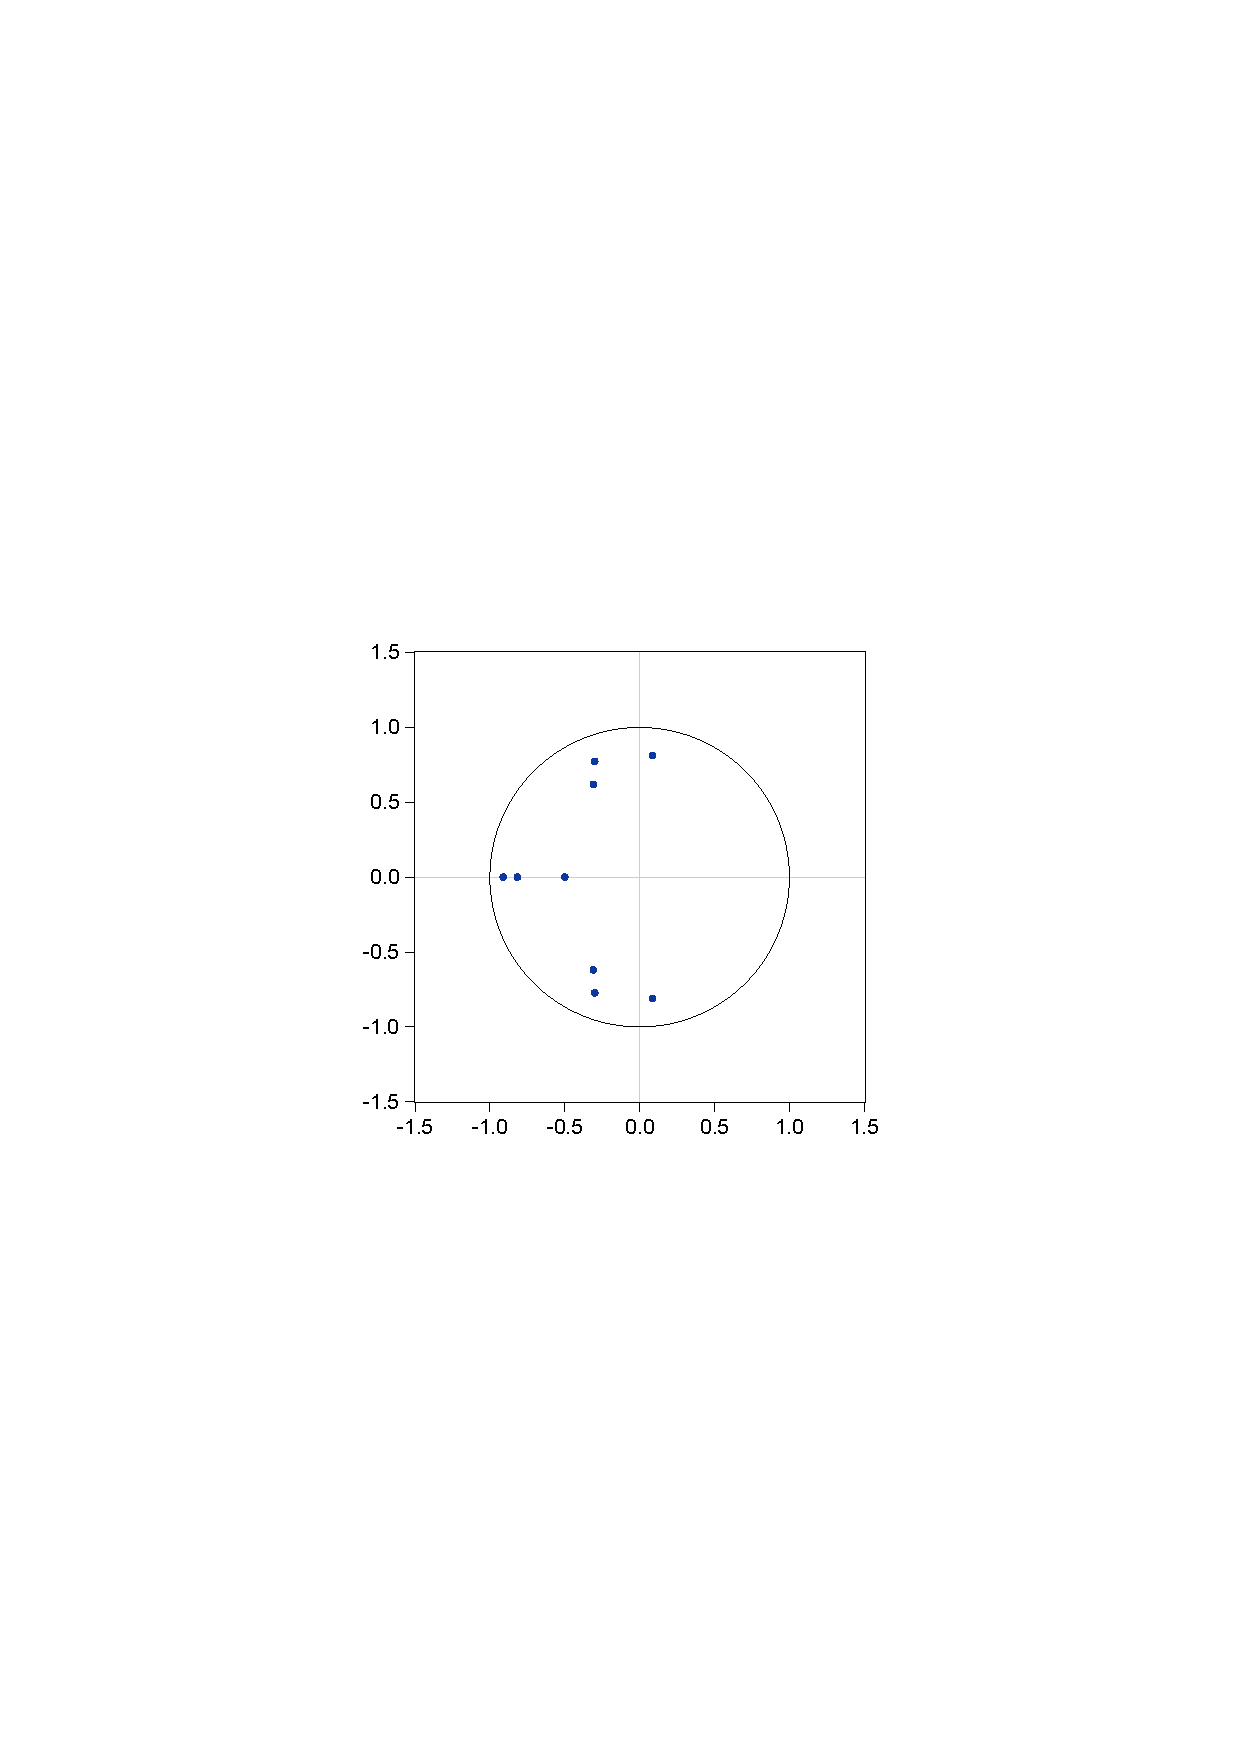
\includegraphics[width=0.6\textwidth]{chap3/arroot.pdf}
    \caption{AR根平稳性检验}
    \label{fig:AR根平稳性检验}
\end{figure}

%%%%%%%%%%%%%%%%%%%%%%%%%%%%%%%%%%%%%%%%%%%%%%%%%%%%%%%%%%%%%%%%%%%
\section{预测模型的应用}

1.采用1号线数据预测2号线束

2.对于外部突发情况适应性高

3.可考虑沉降数据空间关联性

拓扑图

%%%%%%%%%%%%%%%%%%%%%%%%%%%%%%%%%%%%%%%%%%%%%%%%%%%%%%%%%%%%%%%%%%%
\section{本章小结}

正文